% \documentclass[dvipdfmx, 11pt]{beamer}
\documentclass[aspectratio=169, dvipdfmx, 11pt]{beamer} % aspectratio=43, 149, 169
\usepackage{here, amsmath, latexsym, amssymb, bm, ascmac, mathtools, multicol, tcolorbox, subfig}
\usepackage{xcolor}

%デザインの選択(省略可)
\usetheme{Luebeck}
%カラーテーマの選択(省略可)
\usecolortheme{orchid}
%フォントテーマの選択(省略可)
\usefonttheme{professionalfonts}
%フレーム内のテーマの選択(省略可)
\useinnertheme{circles}
%フレーム外側のテーマの選択(省略可)
\useoutertheme{infolines}
%しおりの文字化け解消
\usepackage{atbegshi}
\ifnum 42146=\euc"A4A2
\AtBeginShipoutFirst{\special{pdf:tounicode EUC-UCS2}}
\else
\AtBeginShipoutFirst{\special{pdf:tounicode 90ms-RKSJ-UCS2}}
\fi
%ナビゲーションバー非表示
\setbeamertemplate{navigation symbols}{}
%既定をゴシック体に
\renewcommand{\kanjifamilydefault}{\gtdefault}
%タイトル色
\setbeamercolor{title}{fg=structure, bg=}
%フレームタイトル色
\setbeamercolor{frametitle}{fg=structure, bg=}
%スライド番号のみ表示
%\setbeamertemplate{footline}[frame number]
%itemize
\setbeamertemplate{itemize item}{\small\raise0.5pt\hbox{$\bullet$}}
\setbeamertemplate{itemize subitem}{\tiny\raise1.5pt\hbox{$\blacktriangleright$}}
\setbeamertemplate{itemize subsubitem}{\tiny\raise1.5pt\hbox{$\bigstar$}}
% color
\newcommand{\red}[1]{\textcolor{red}{#1}}
\newcommand{\green}[1]{\textcolor{green!40!black}{#1}}
\newcommand{\blue}[1]{\textcolor{blue!80!black}{#1}}

% (Useful) Sets
\newcommand{\NaturalNumberSet}{\mathbb{N}}
\newcommand{\RealNumberSet}{\mathbb{R}}
\newcommand{\NDemenstionalRealEuclideanSpace}{\mathbb{R}^n}

% Symbols
\newcommand{\Epigraph}[1]{\text{epi\:${#1}$}} % epi
% (Useful) Texts
\newcommand{\SuchThat}{\:\text{s.t.}\:}
\newcommand{\Painleve}{Painlev\'e}

% Set form e.g. {x | ...}
% #1: element
% #2: conditions
\newcommand{\SetForm}[2]{
  \{{#1}\:|\:{#2}\}
}

\title[博士後期課程入学試験]{集合値写像における Asymptotic Functions}
\author[岩本 崚汰]{岩本 崚汰*, 田中 環}
\institute[新潟大学大学院自然科学研究科]{新潟大学大学院自然科学研究科}
\date{2023年08月22日}

\titlegraphic{
\includegraphics[keepaspectratio, scale=0.20]{figures/niigata_university_logo.png}}

\begin{document}
\maketitle

\begin{frame}{Contents}
  \tableofcontents
\end{frame}

% 1.準備
% ----------------------------------------------------------------
\section{準備}
\begin{frame}{内容}
  \tableofcontents[currentsection]
\end{frame}

% 1.1
\begin{frame}{準備(1)}
  今回主に扱うのは $\mathbb{R}^n$ の実ベクトル空間とする。

  また、内積は以下のように定義する。

  \begin{equation}
    x=(x_1,\dots,x_n)^T, y=(y_1,\dots,y_n)^T \in \mathbb{R}^n, \left\langle x,y\right\rangle \coloneqq \sum_{i = 1}^{n} x_i y_i. \notag
  \end{equation}

  ノルムに関しては、$\left\lVert x \right\rVert \coloneqq \left\langle x,x\right\rangle ^{1/2} $ とする。
\end{frame}

% 1.2
\begin{frame}{準備(2)}
  \begin{block}{定義 1 (Proper) \cite{ref1}}
    $f: \NDemenstionalRealEuclideanSpace \rightarrow \RealNumberSet \cup \{\pm \infty\}$ に対して以下の2つが成り立つ時、$f$ は proper であるという。
    \begin{enumerate}
      \item $\exists x \in \NDemenstionalRealEuclideanSpace \SuchThat f(x) < \infty$,
      \item $\forall x \in \NDemenstionalRealEuclideanSpace, f(x) > -\infty$.
    \end{enumerate}
  \end{block}

  \begin{block}{定義 2 (Epigraph) \cite{ref1}}
    $f: \NDemenstionalRealEuclideanSpace \rightarrow \RealNumberSet \cup \{\pm \infty\}$ に対して、以下の集合 $\Epigraph{f}$ を $f$ の epigraph という。

    \begin{equation}
      \Epigraph{f} \coloneqq \SetForm{(x,t) \in \NDemenstionalRealEuclideanSpace \times \RealNumberSet}{f(x) \leq t}. \notag
    \end{equation}
  \end{block}
\end{frame}

% 2.Asymptotic Cones
% ----------------------------------------------------------------
\section{Asymptotic Cones}
\begin{frame}{Contents}
  \tableofcontents[currentsection]
\end{frame}

% 2.1
\begin{frame}{``Asymptotic'' とは}
  \pause
  $\rightarrow$ ある対象を無限に離れた位置から観測する過程のこと。

  \medskip

  \centering
    \begin{columns}
      \pause
      \begin{column}{0.48\textwidth}
      \centering
      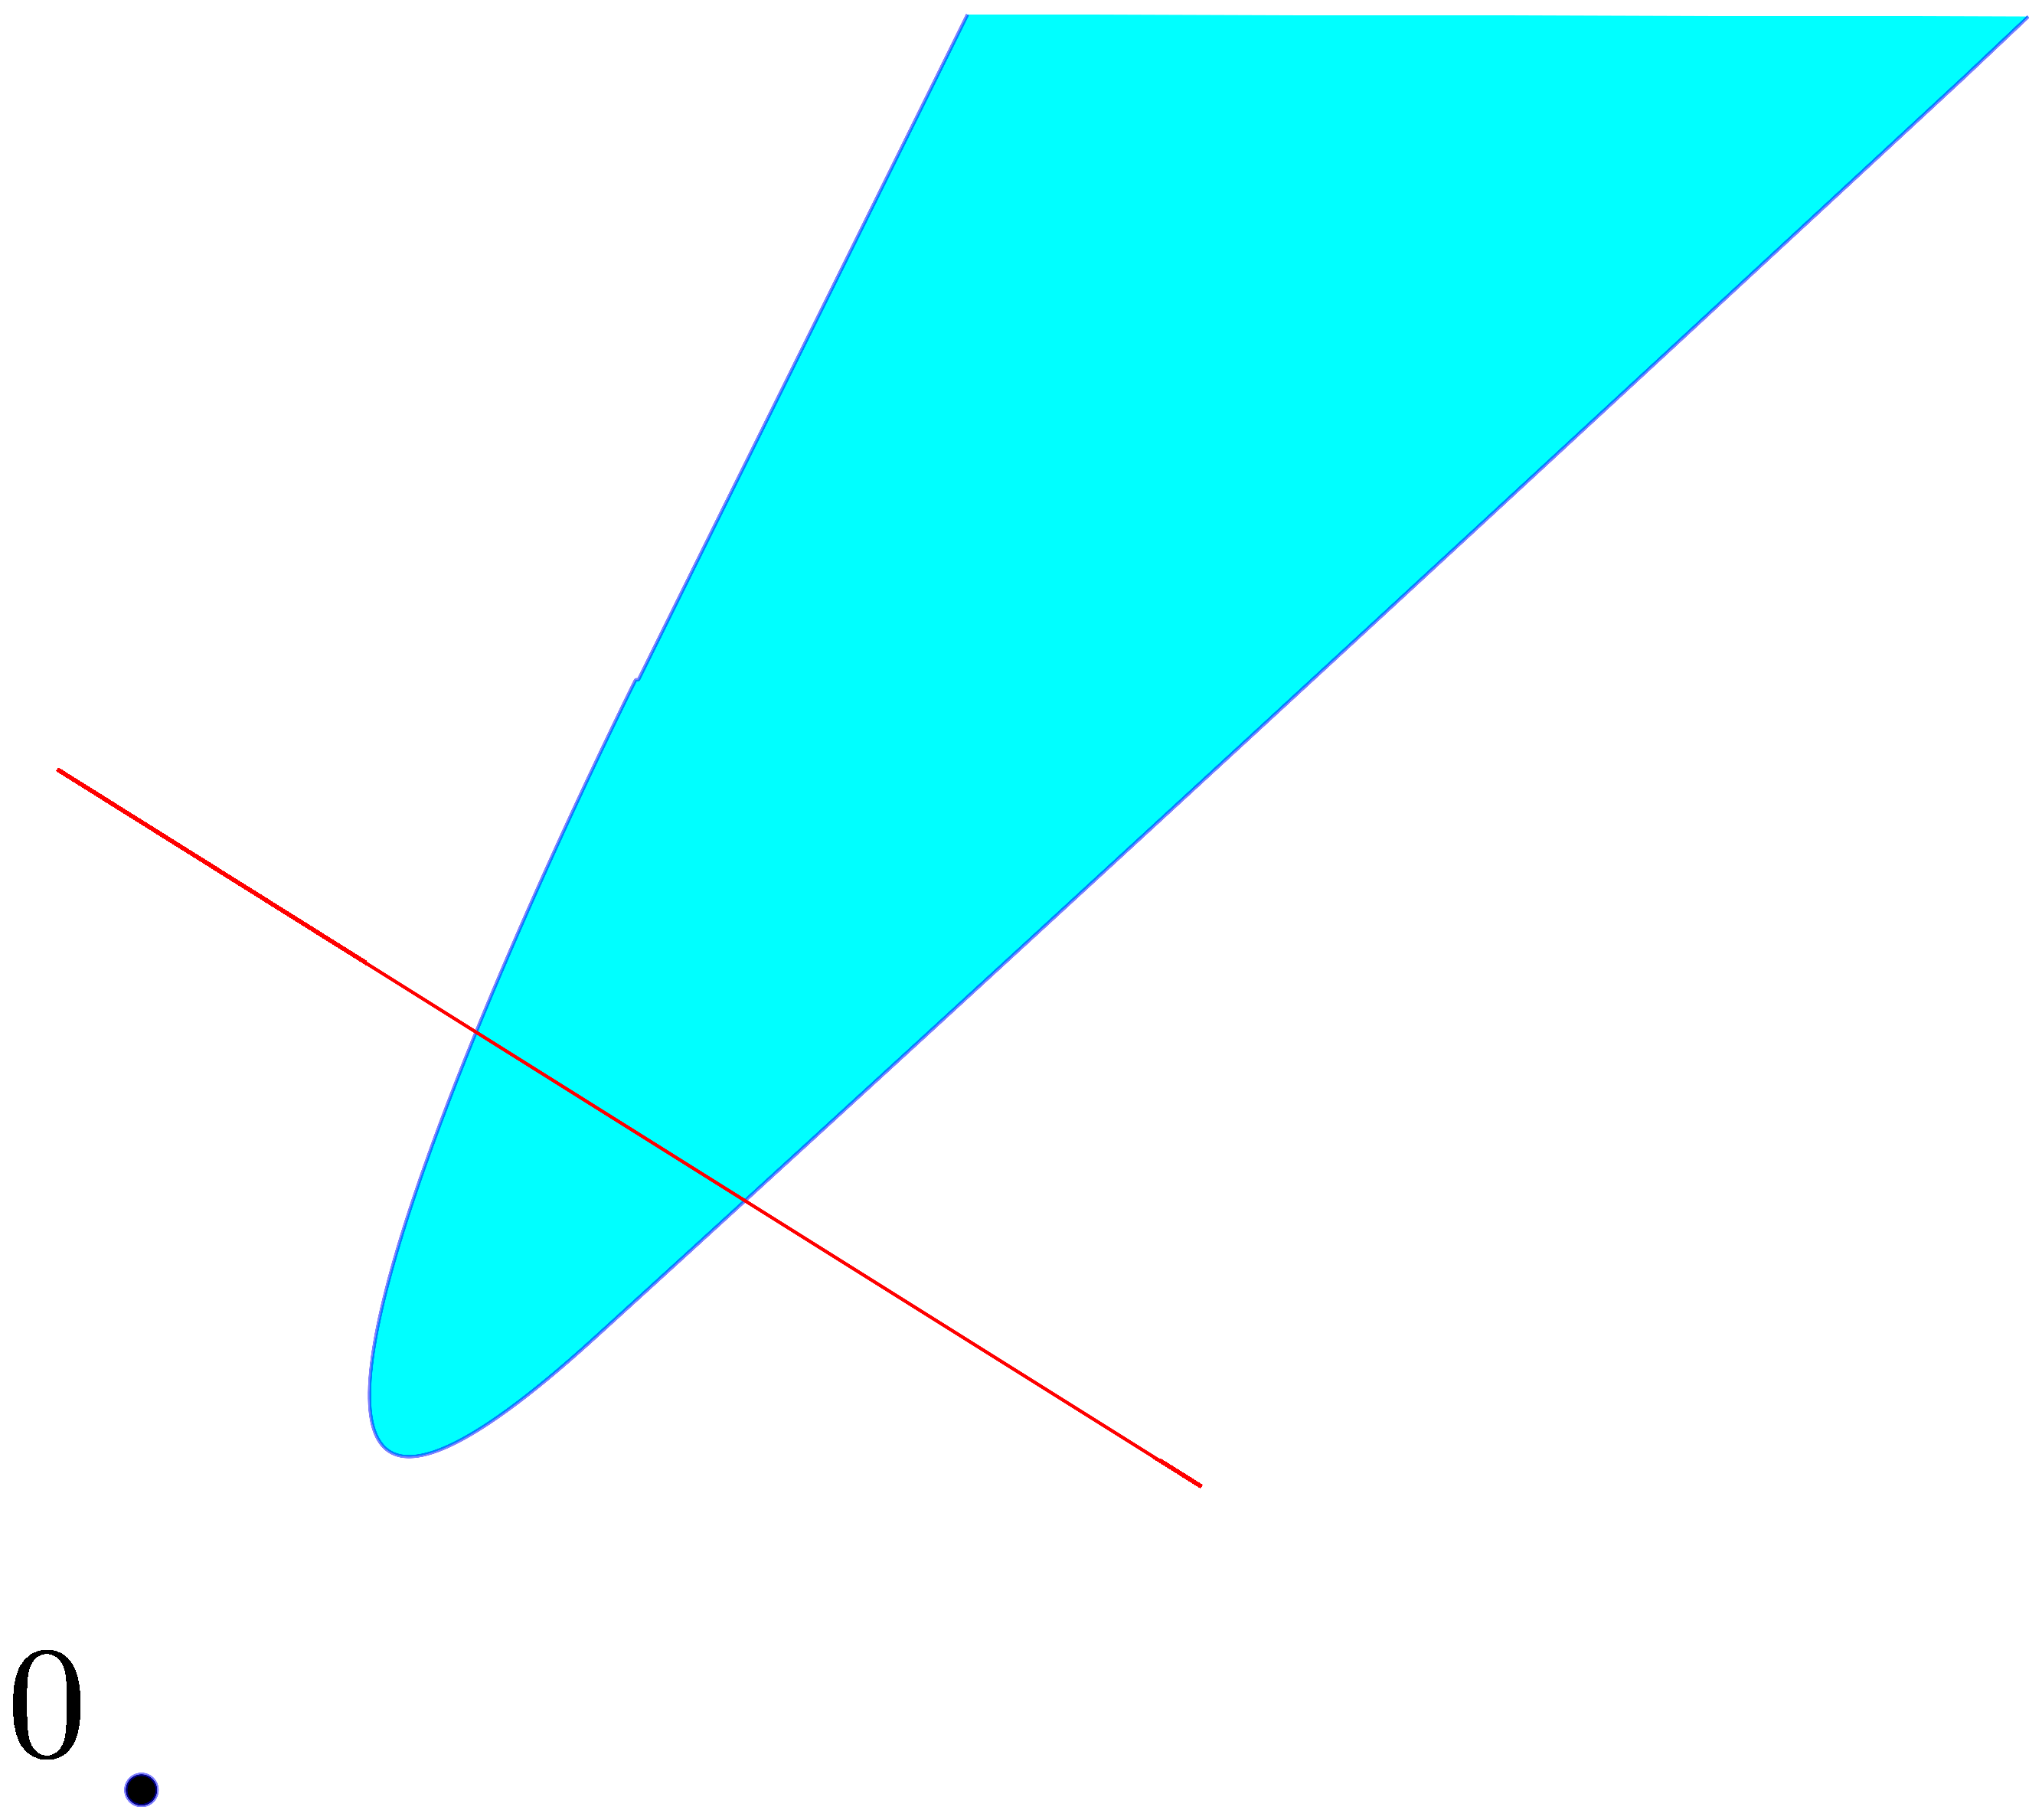
\includegraphics[keepaspectratio, scale=0.095]{figures/asymptotic_meaning_1.eps}
      \end{column}
      \pause
      \begin{column}{0.48\textwidth}
      \centering
      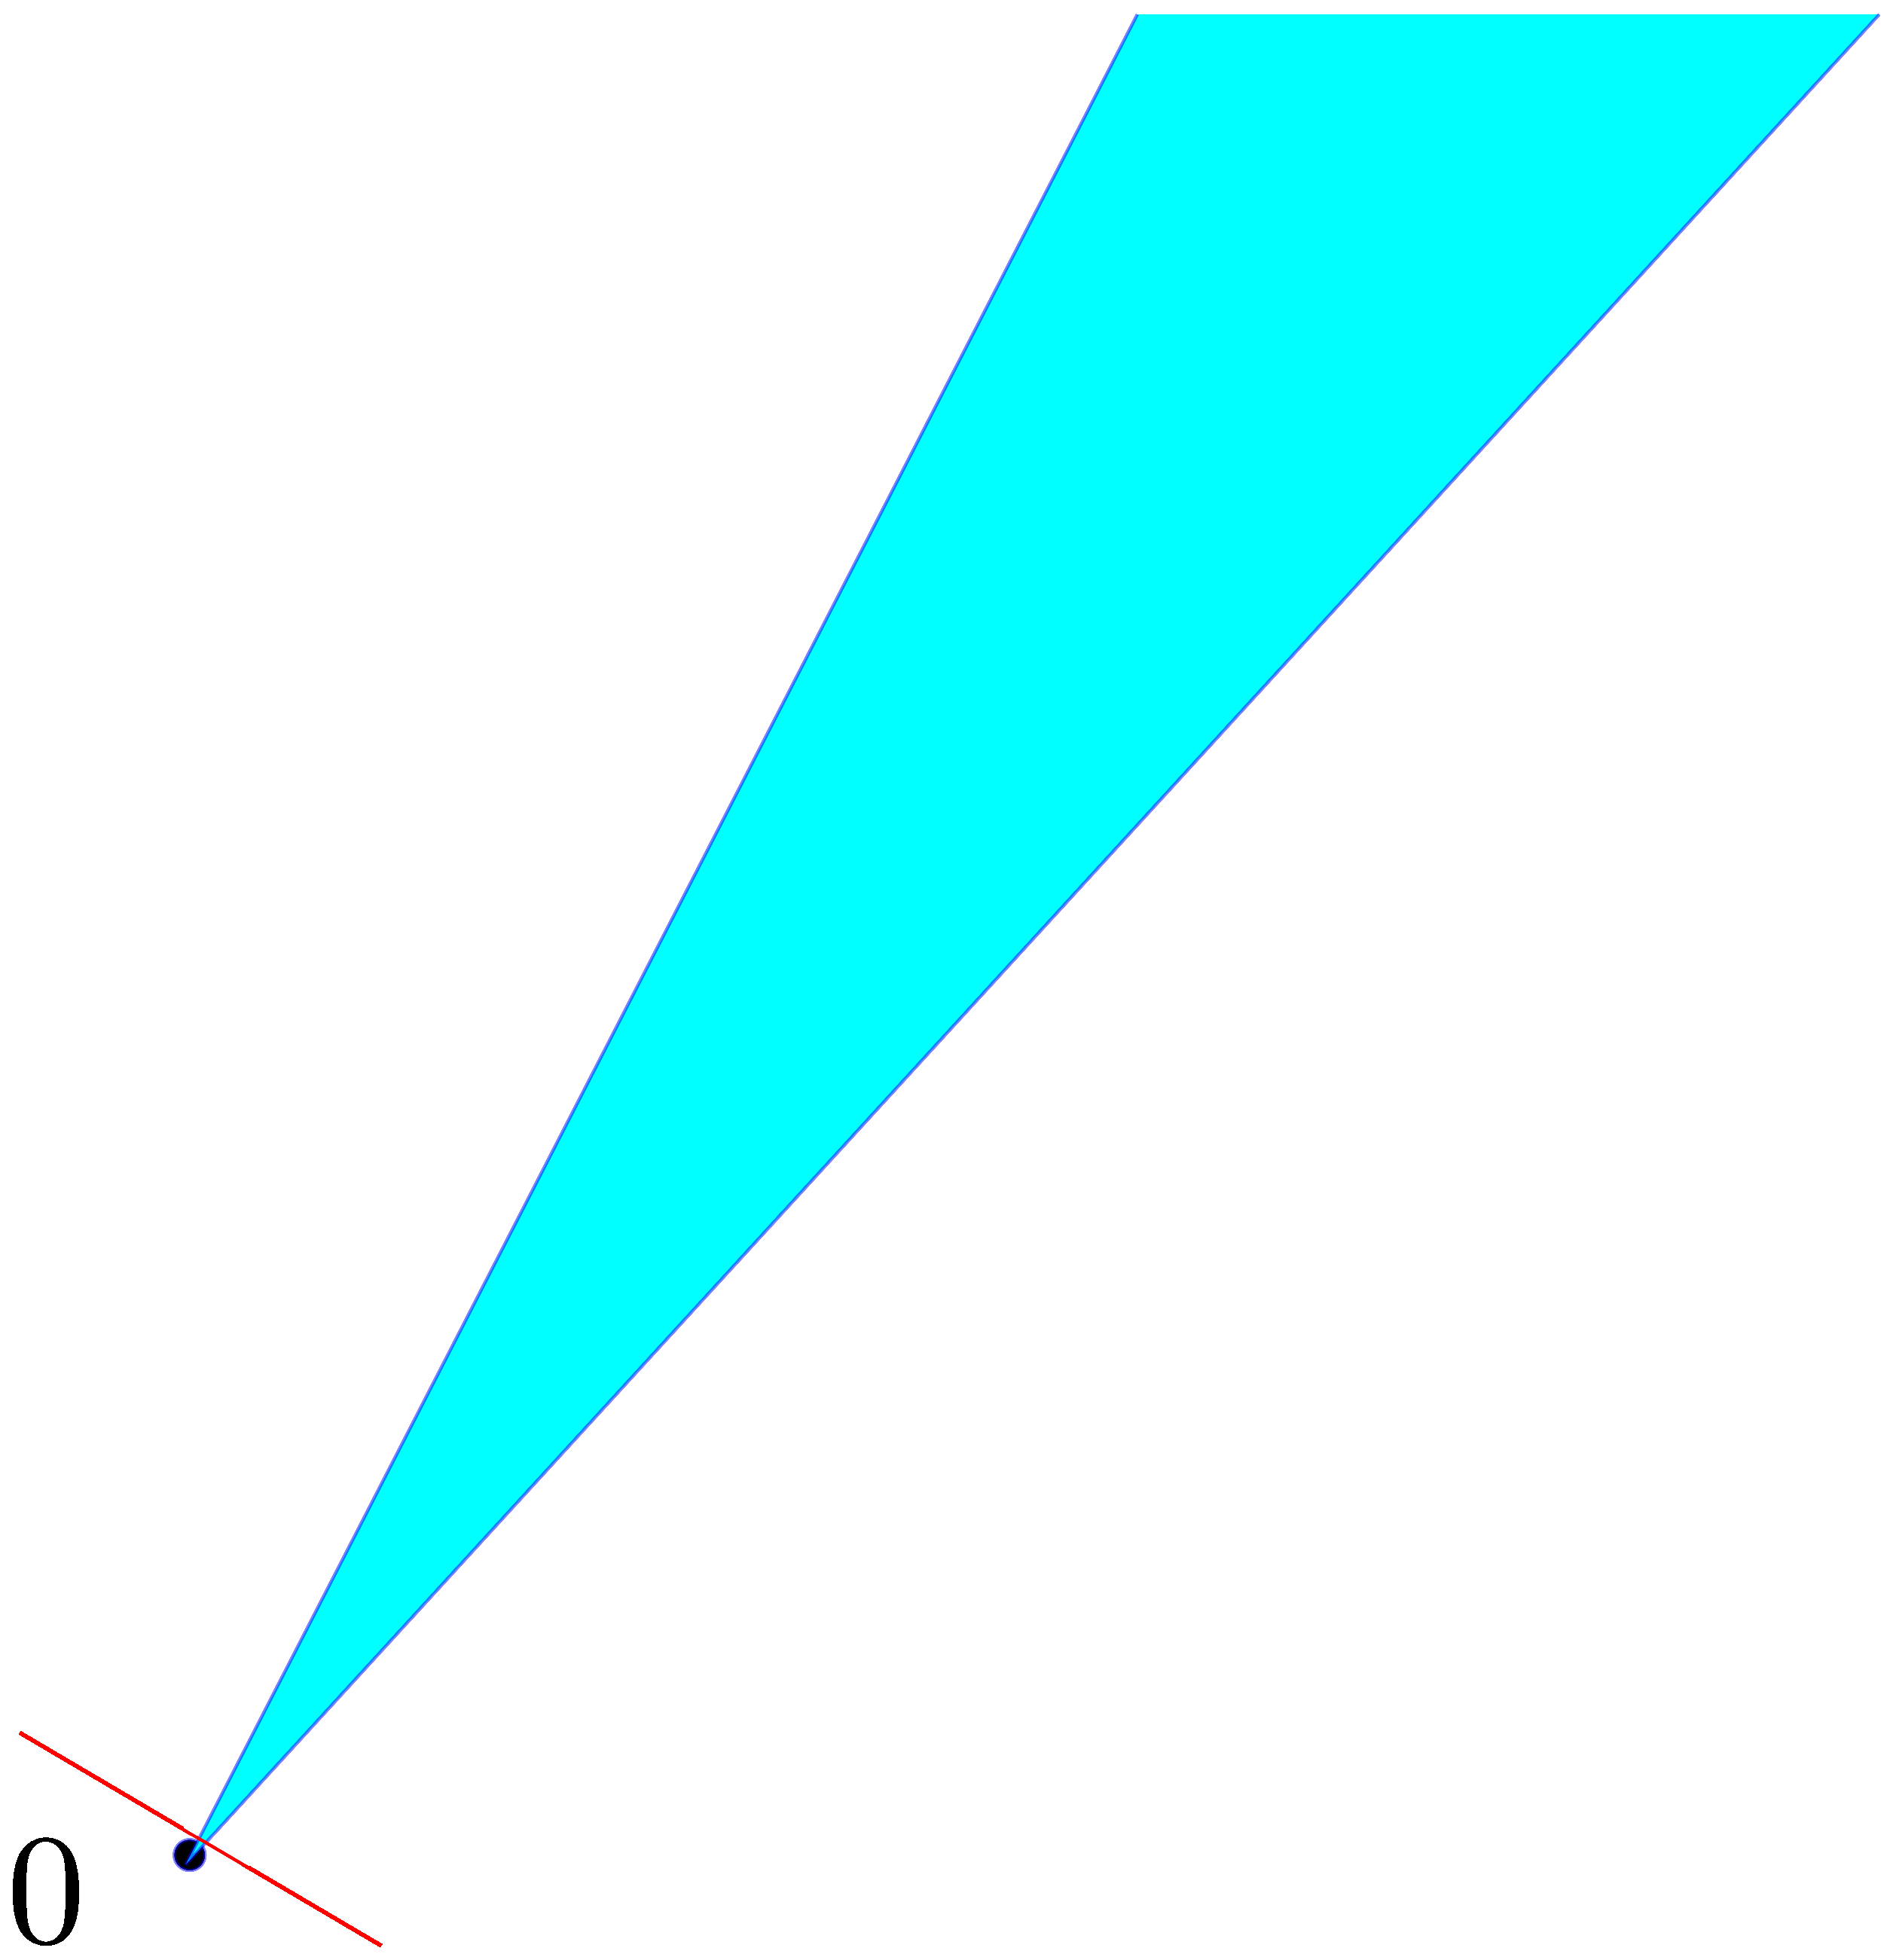
\includegraphics[keepaspectratio, scale=0.095]{figures/asymptotic_meaning_2.eps}
    \end{column}
  \end{columns}
\end{frame}

% 2.2
\begin{frame}{Asymptotic Cones の定義}
  \begin{block}{定義 3 (Asymptotic Cones) \cite{ref1}}
    $C \subset \mathbb{R}^n$, $C \ne \emptyset$ とする。このとき$C$ の asymptotic cone、記号で $C_\infty$ 、は点列 $\{ x_k \} \subset C$ を用いて以下のように定義する。
    \begin{equation}
    C_\infty = \left\{ d \in
    \mathbb{R}^n \:\middle|\: \exists t_k \rightarrow +\infty, \exists x_k \in C \:\text{with}\: \lim_{k \to \infty} \frac{x_k}{t_k} = d \right\}. \notag
    \end{equation}
  \end{block}

  \pause
  Example: $C = \{(x,y) \in \mathbb{R}^2 \:|\: y=x^2\}$. We let $\textcolor{blue}{x_k} = (k, k^2)$ and $t_k = \left\lVert x_k \right\rVert$.

  \centering
  \begin{columns}
    \pause
    \begin{column}{0.48\textwidth}
    \centering
    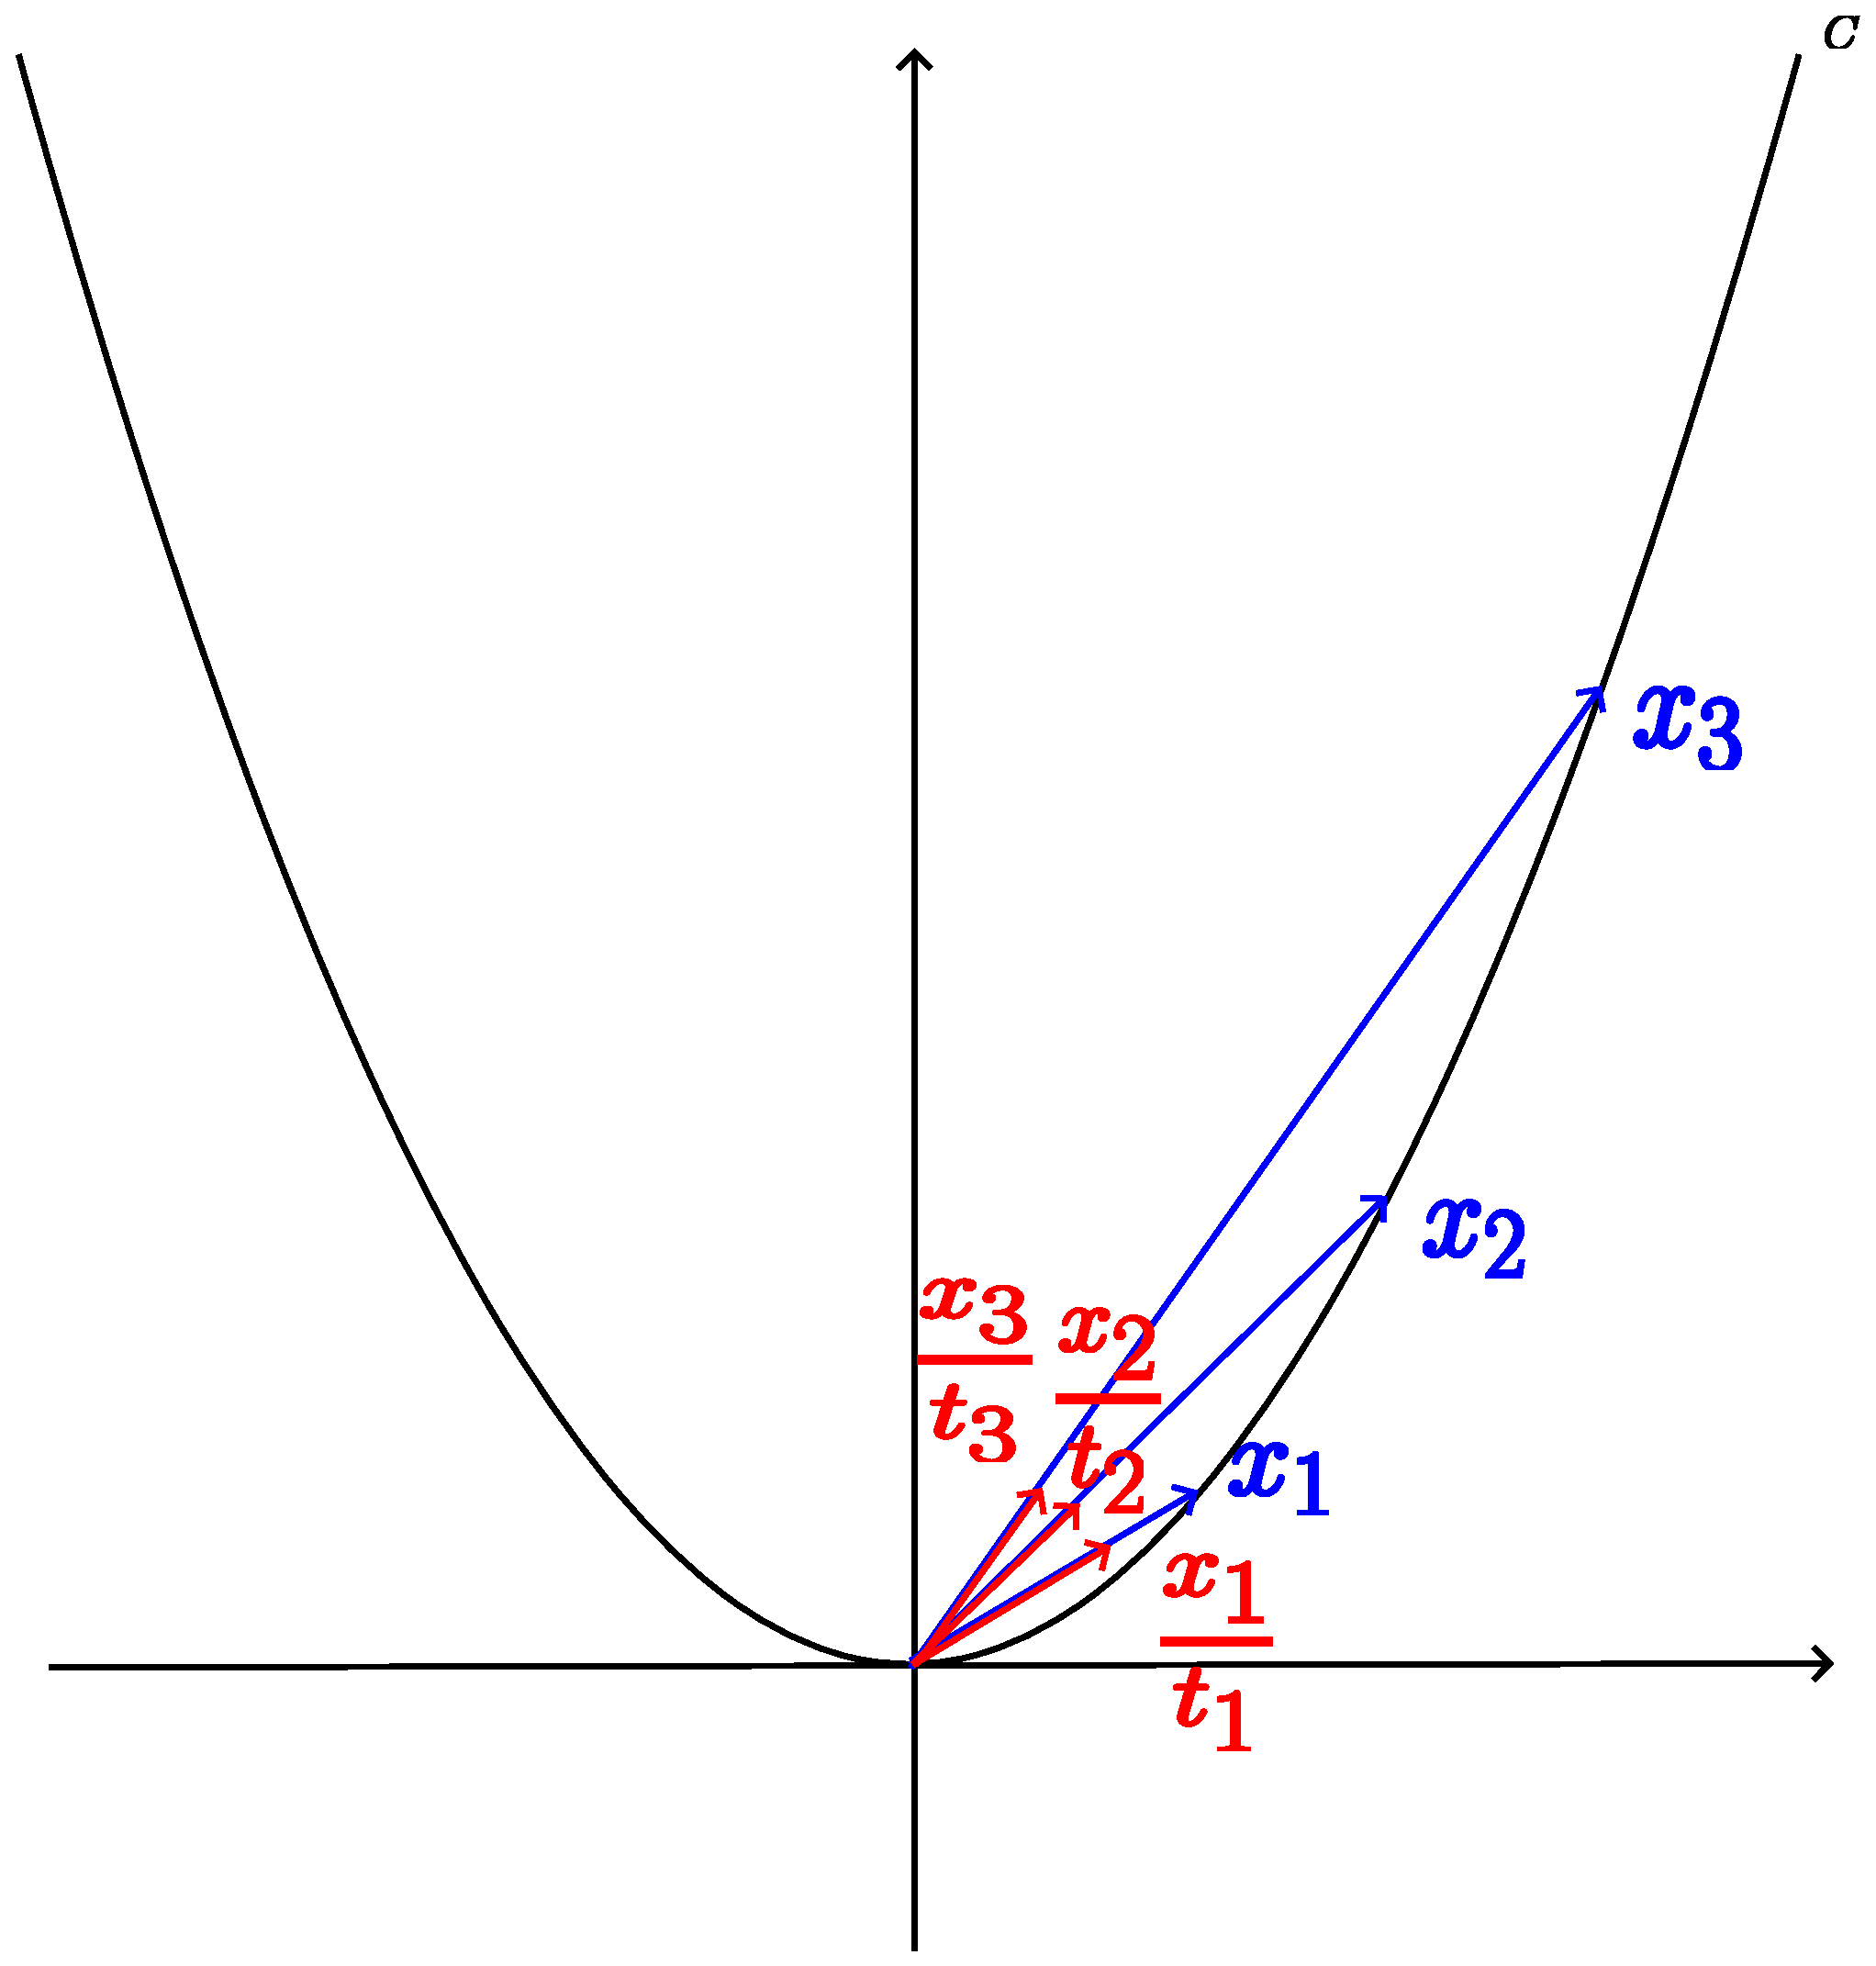
\includegraphics[keepaspectratio, scale=0.095]{figures/figure_asymptotic_cone_1.eps}
    \end{column}
    \pause
    \begin{column}{0.48\textwidth}
    \centering
    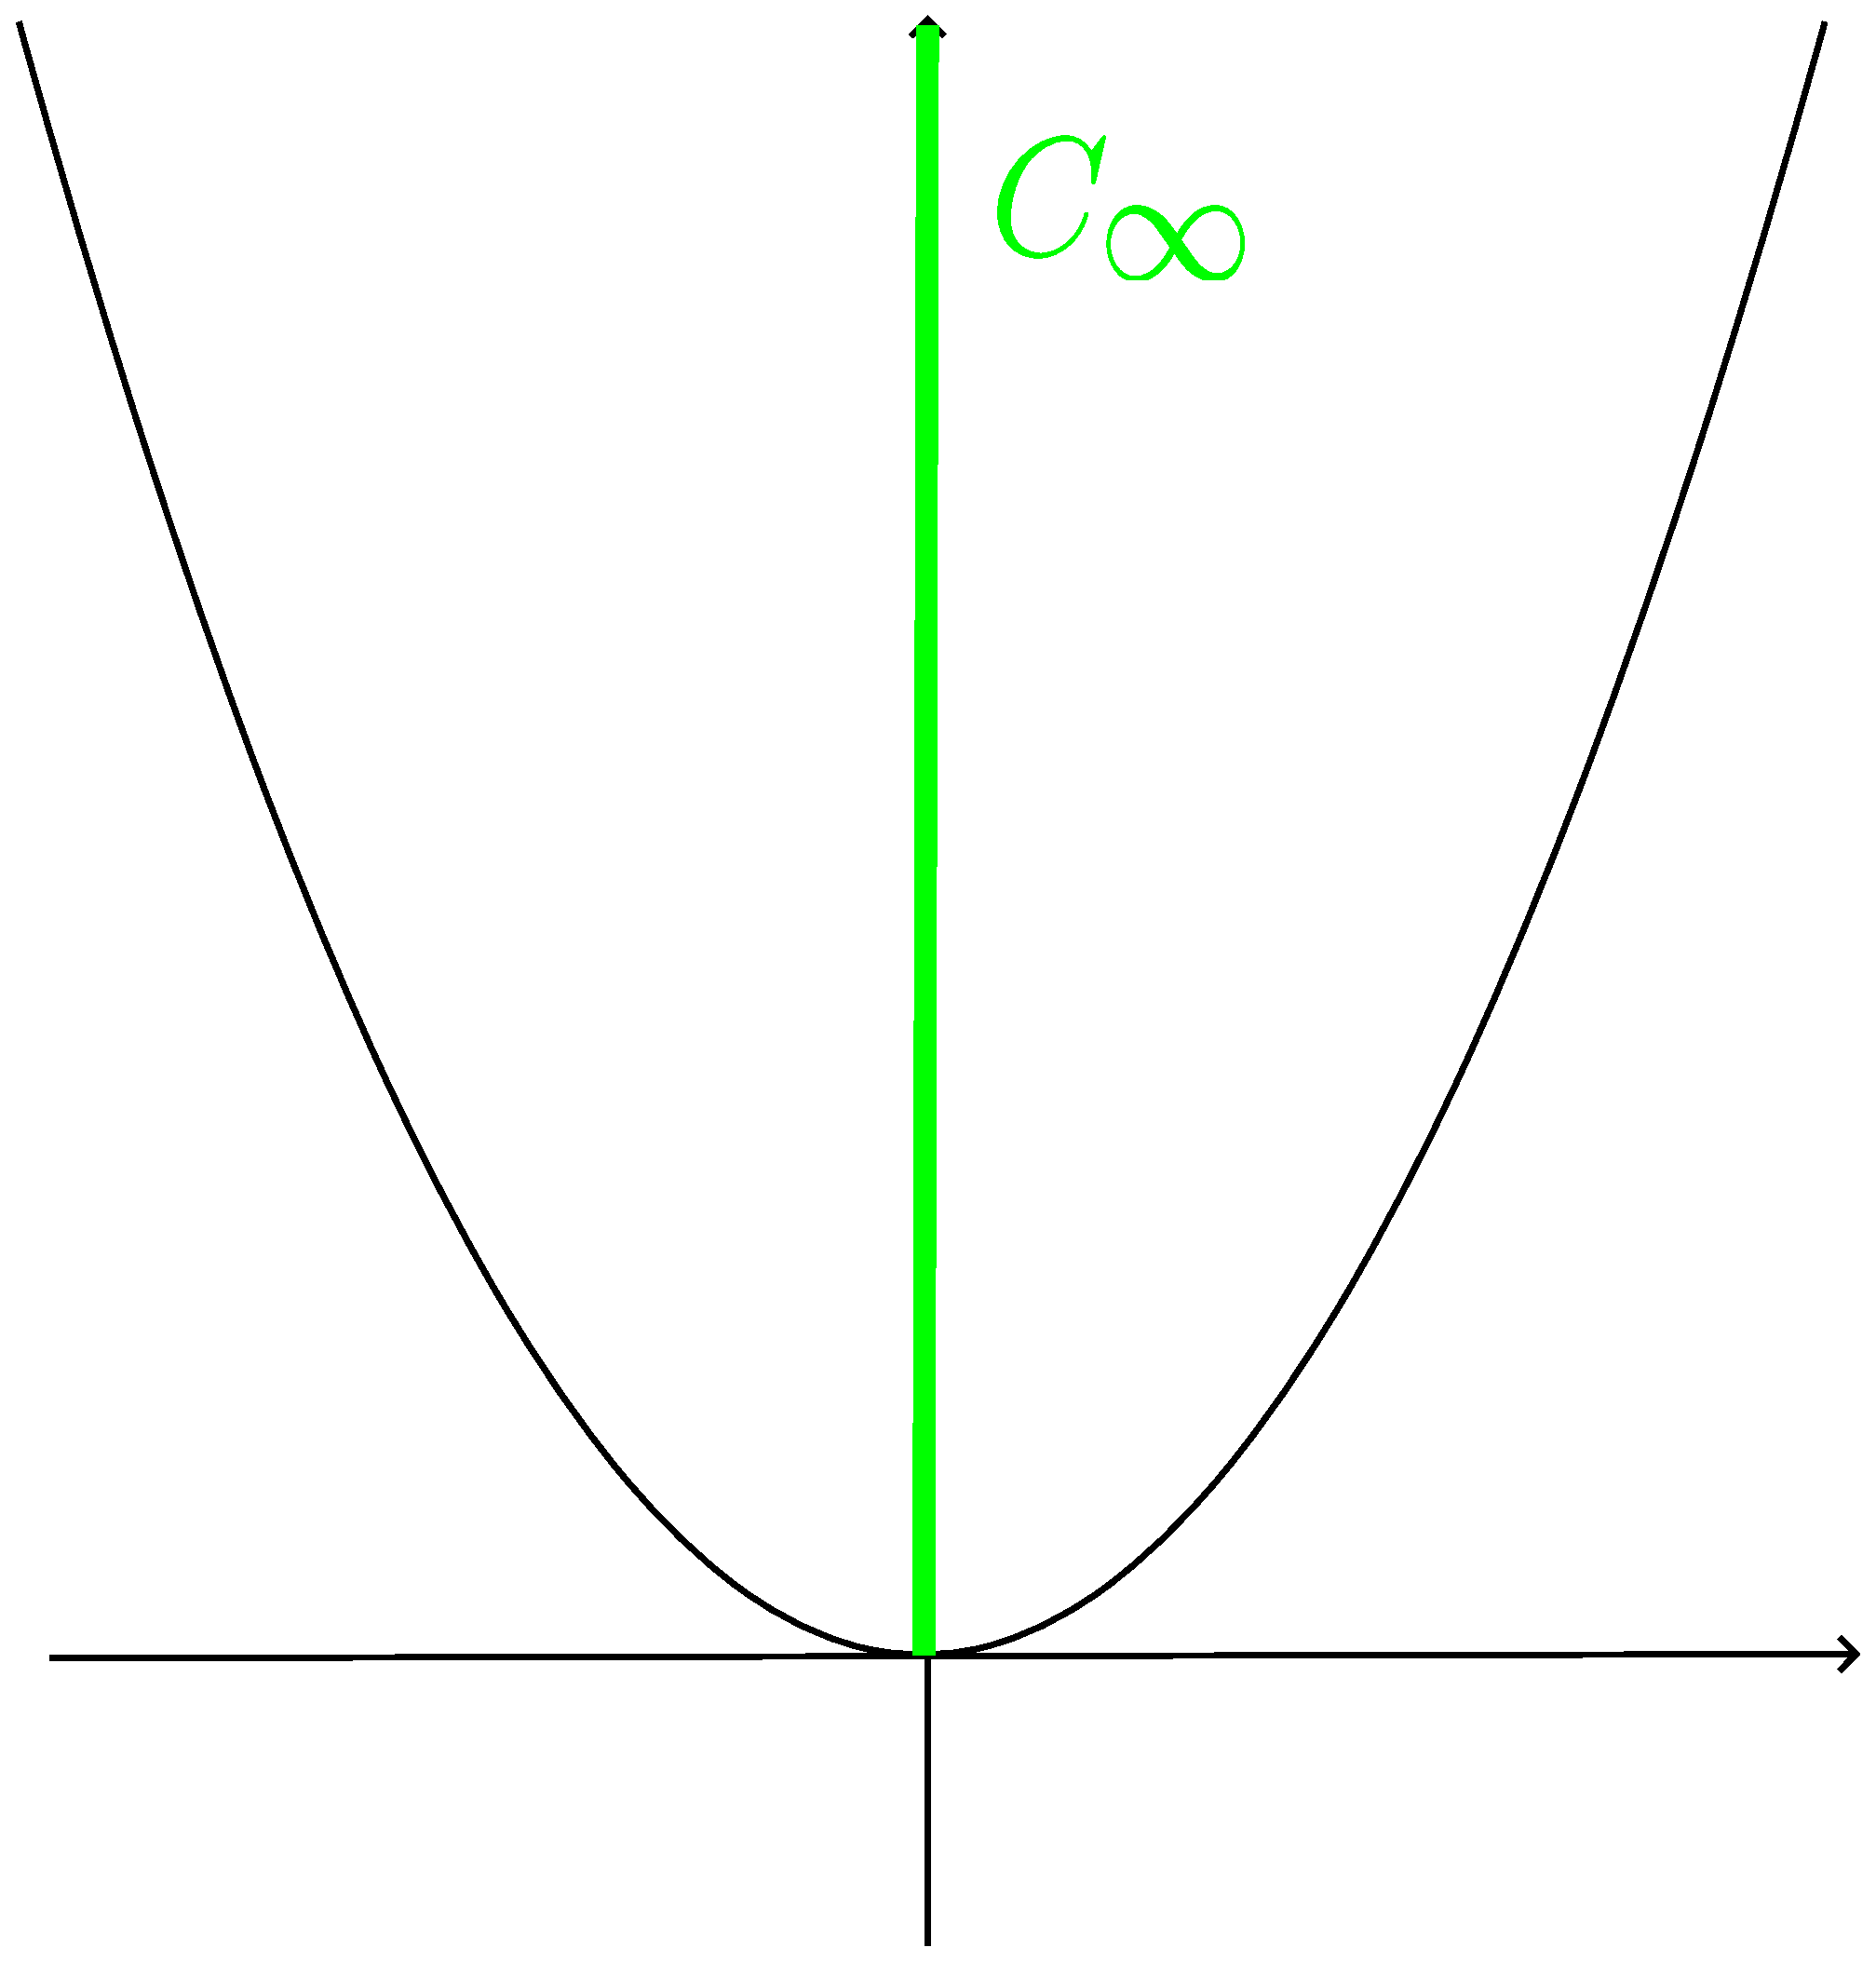
\includegraphics[keepaspectratio, scale=0.095]{figures/figure_asymptotic_cone_2.eps}
    \end{column}
  \end{columns}
\end{frame}

% 3.Asymptotic Functions
% ----------------------------------------------------------------
\section{Asymptotic Functions}
\begin{frame}{内容}
  \tableofcontents[currentsection]
\end{frame}

% 3.1
\begin{frame}{Asymptotic Functions の定義}
  \begin{block}{定義 4 (Asymptotic Functions) \cite{ref1}}
    $f: \NDemenstionalRealEuclideanSpace \rightarrow \RealNumberSet \cup \{+\infty\}$, proper とする。
    この時、$f$ に対して $\Epigraph{f_{\infty}} = (\Epigraph{f})_{\infty}$ を満たす $f_{\infty}: \NDemenstionalRealEuclideanSpace \rightarrow \RealNumberSet \cup \{+\infty\}$ がただ一つ存在し、この関数 $f_{\infty}$ を asymptotic function と呼ぶ。
  \end{block}

  \pause
  \begin{alertblock}{注意 1 (Asymptotic Functions の作成の流れ)}
    具体的に、ある関数に対しての asymptotic function を求めるには以下の手順を踏む。
    \begin{enumerate}
      \item $f$ の定義
      \item $\Epigraph{f}$ の取得
      \item $(\Epigraph{f})_{\infty}$ の取得
      \item $f_{\infty}$ の定義
    \end{enumerate}
  \end{alertblock}
\end{frame}

% 3.2
\begin{frame}{Asymptotic Functions の作成の流れ}
  Example:
  % 具体例の関数
  % \begin{equation}
  %   f(x) =
  %   \begin{cases}
  %     +\infty, & \text{if $x < 0 $} \\
  %     x^2, & \text{if $0 \leq x \leq 1 $} \\
  %     2x - 1, & \text{if $x > 1 $}
  %   \end{cases} \notag
  % \end{equation}

  \begin{figure}[htbp]
    \begin{tabular}{cc}
      \begin{minipage}[t]{0.45\hsize}
        \centering
        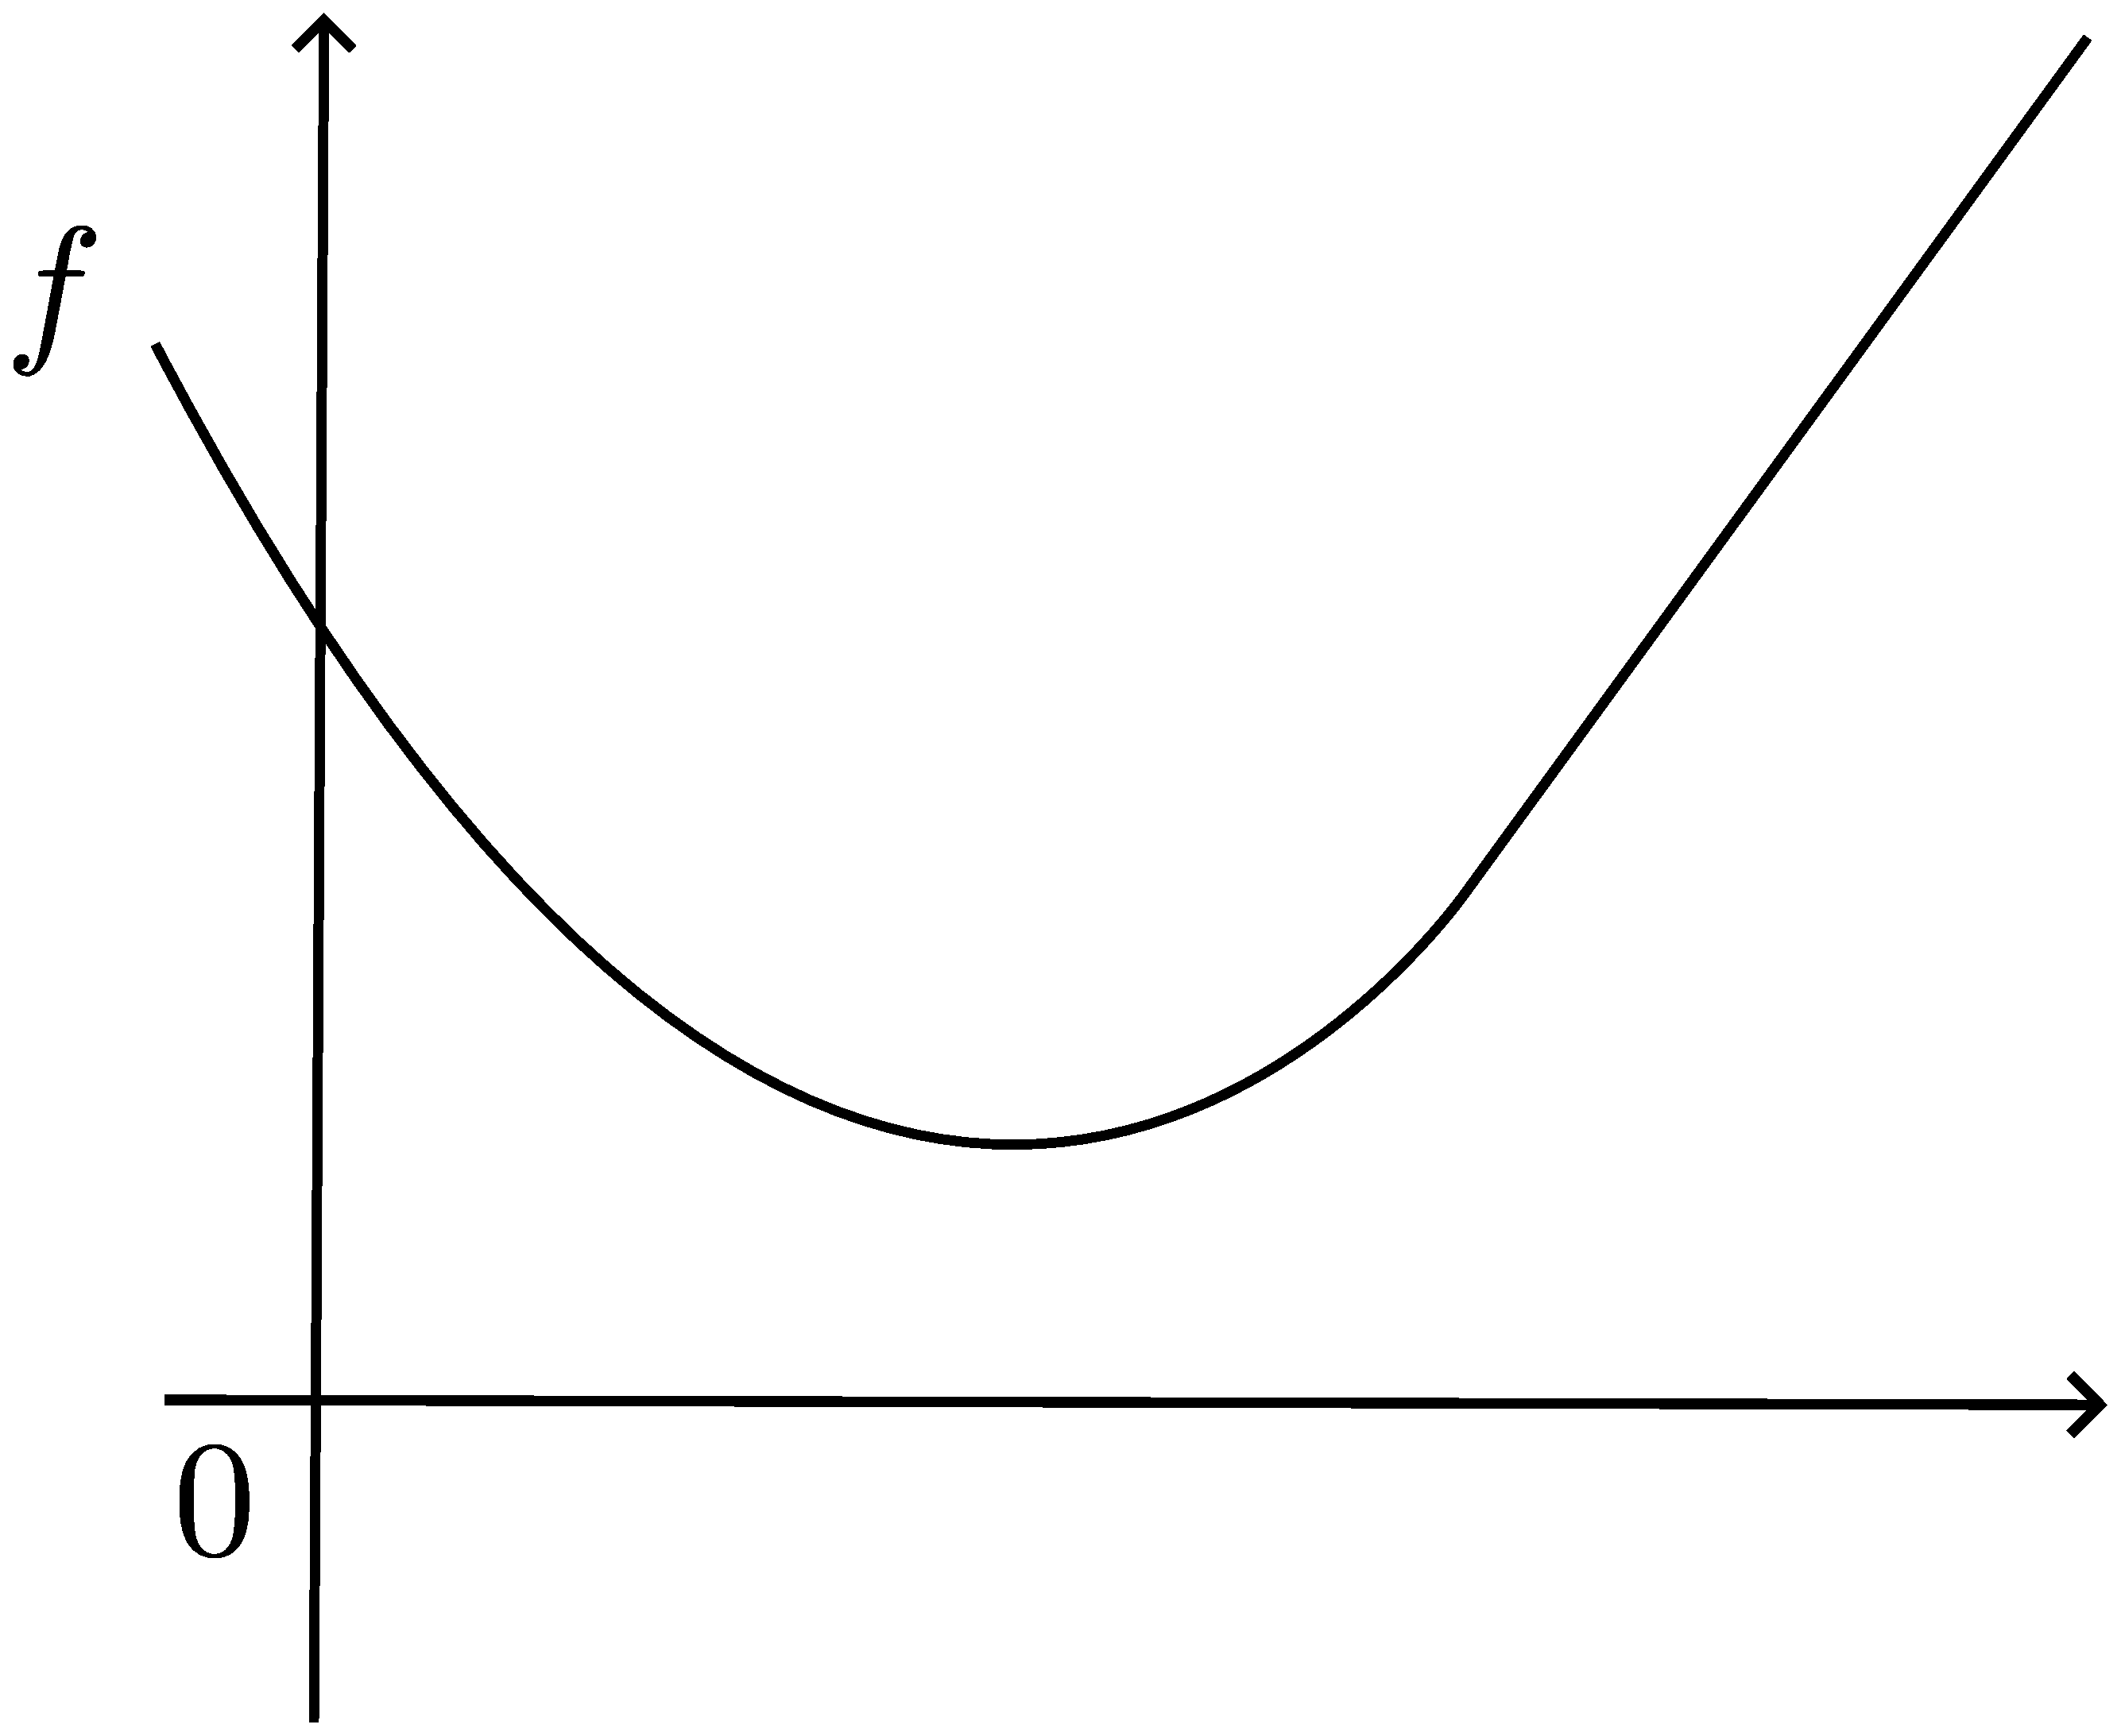
\includegraphics[keepaspectratio, scale=0.07]{figures/asymptotic_function_def/graph_base.eps}
        \caption{(1) $f$ の定義}
        \label{composite}
      \end{minipage} &
      \begin{minipage}[t]{0.45\hsize}
        \centering
        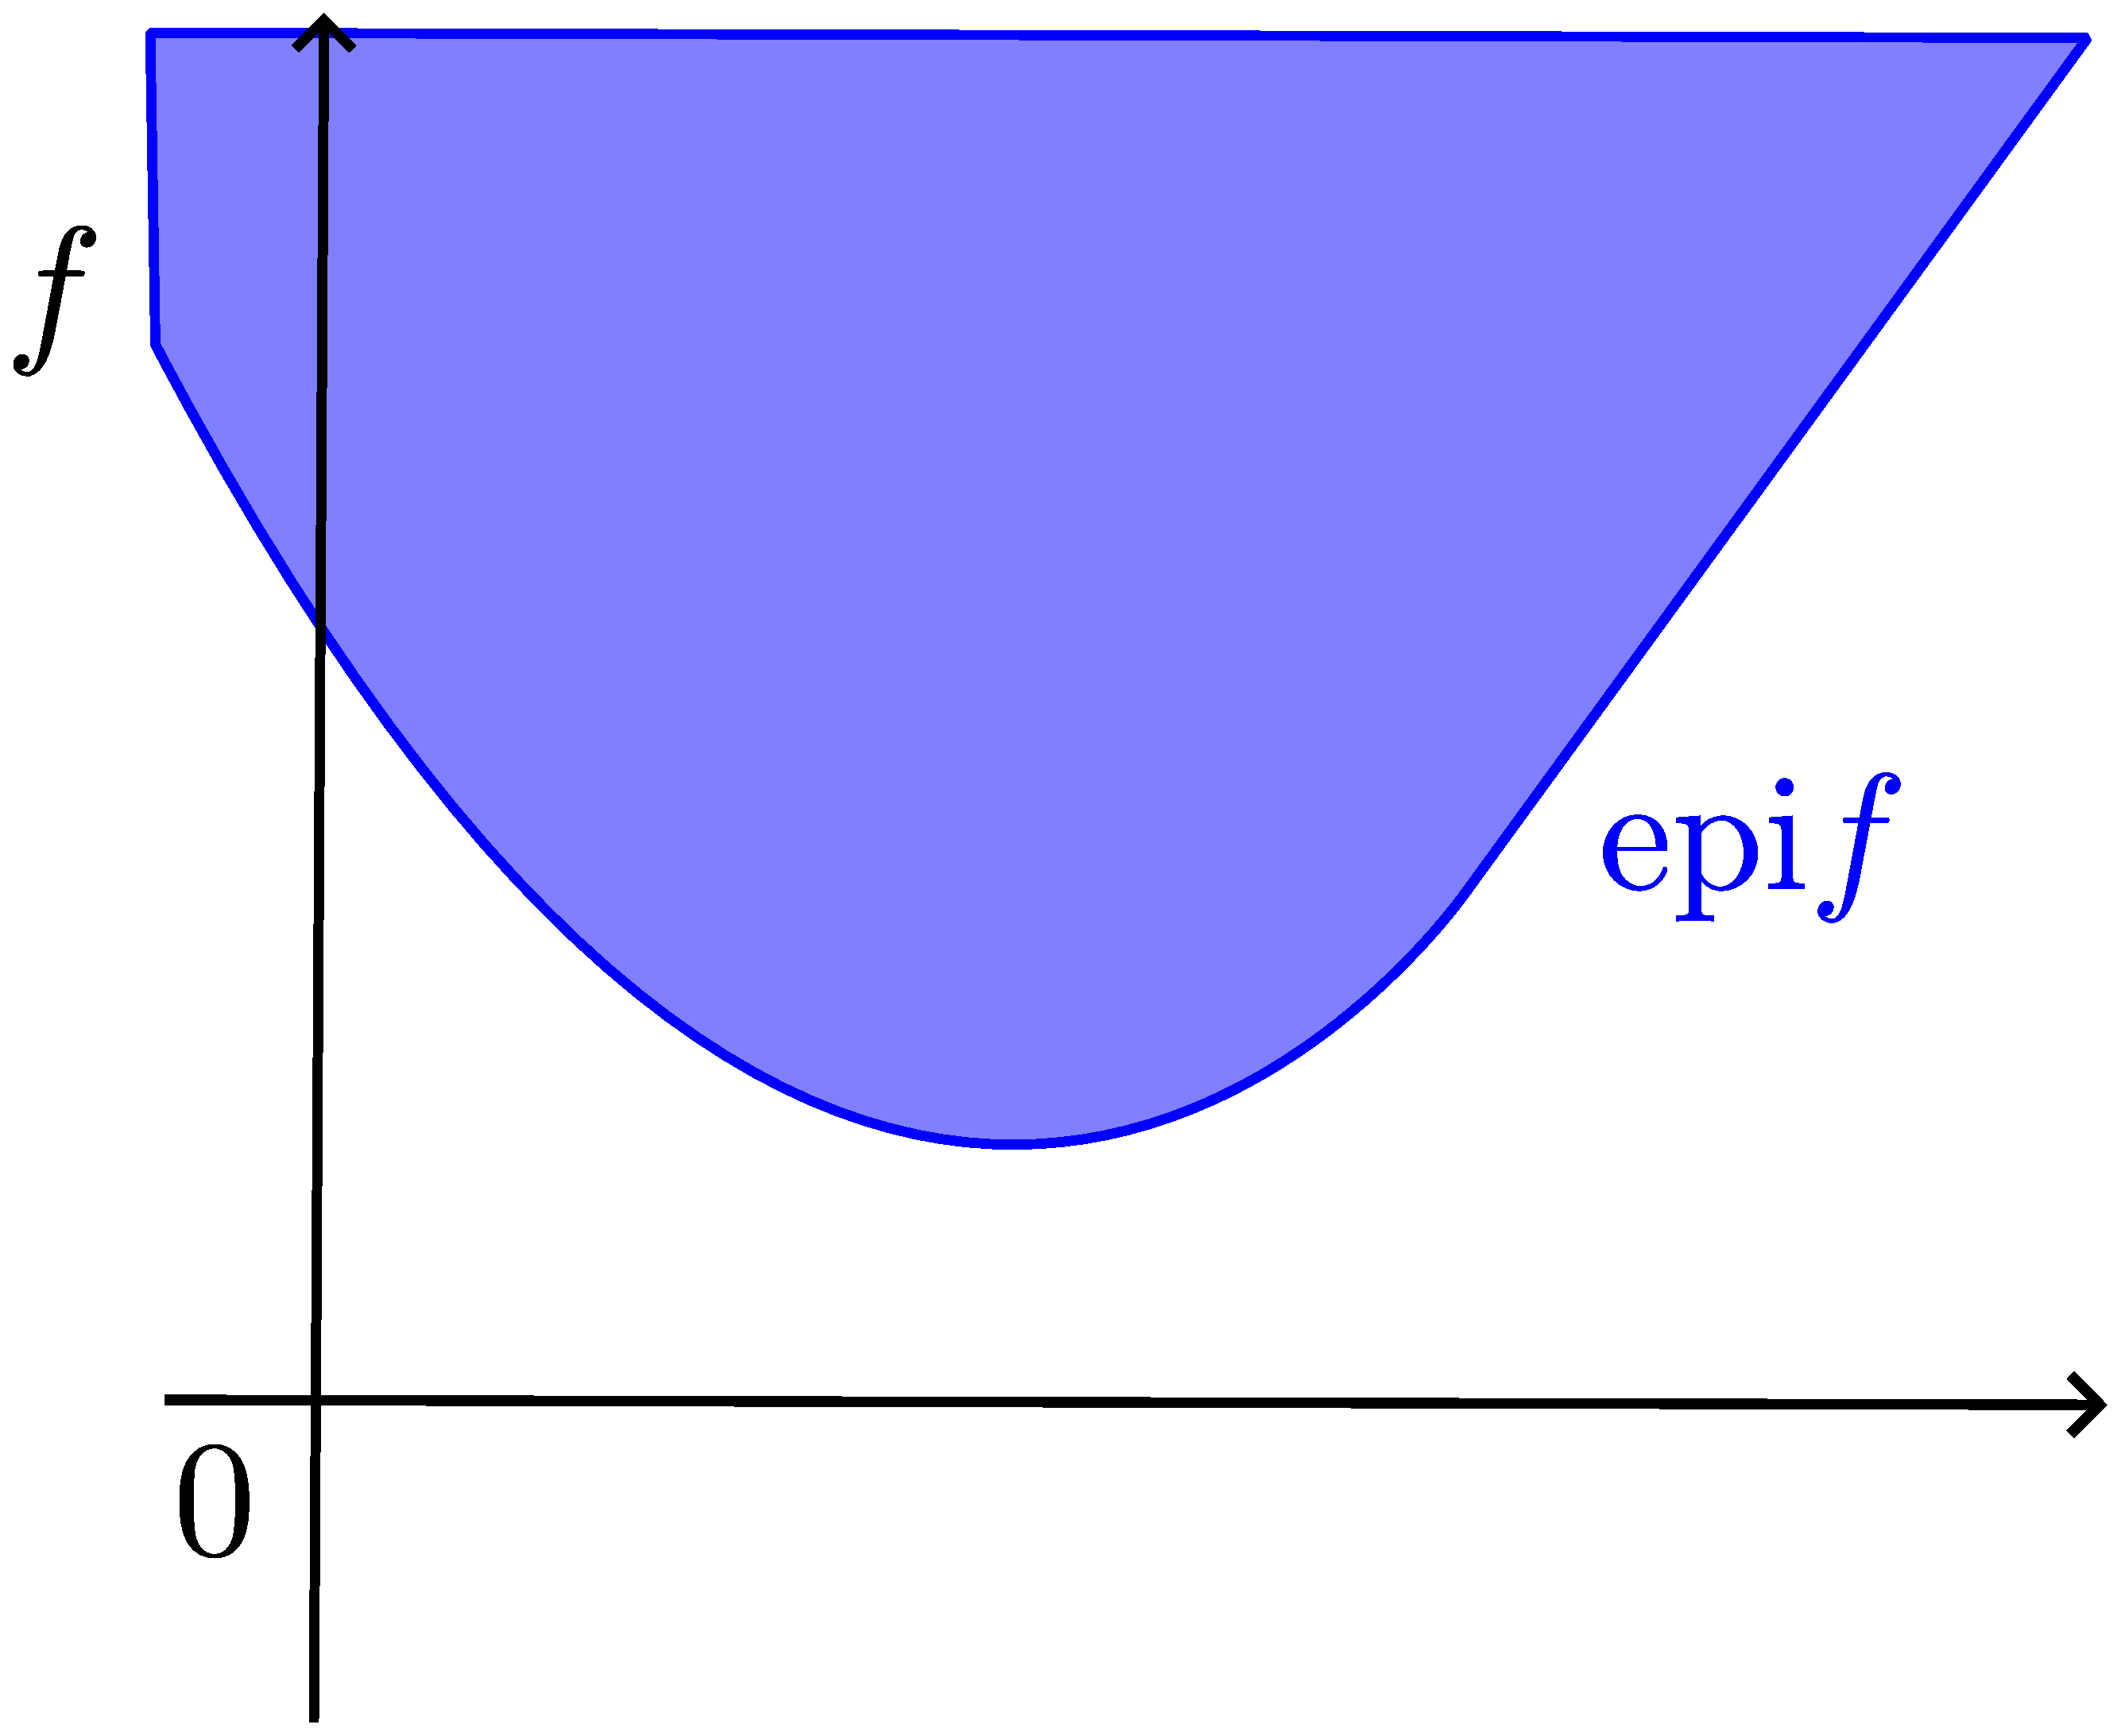
\includegraphics[keepaspectratio, scale=0.07]{figures/asymptotic_function_def/asymptotic_function_epigraph.eps}
        \caption{(2) $\Epigraph{f}$ の取得}
        \label{Gradation}
      \end{minipage} \\

      \begin{minipage}[t]{0.45\hsize}
        \centering
        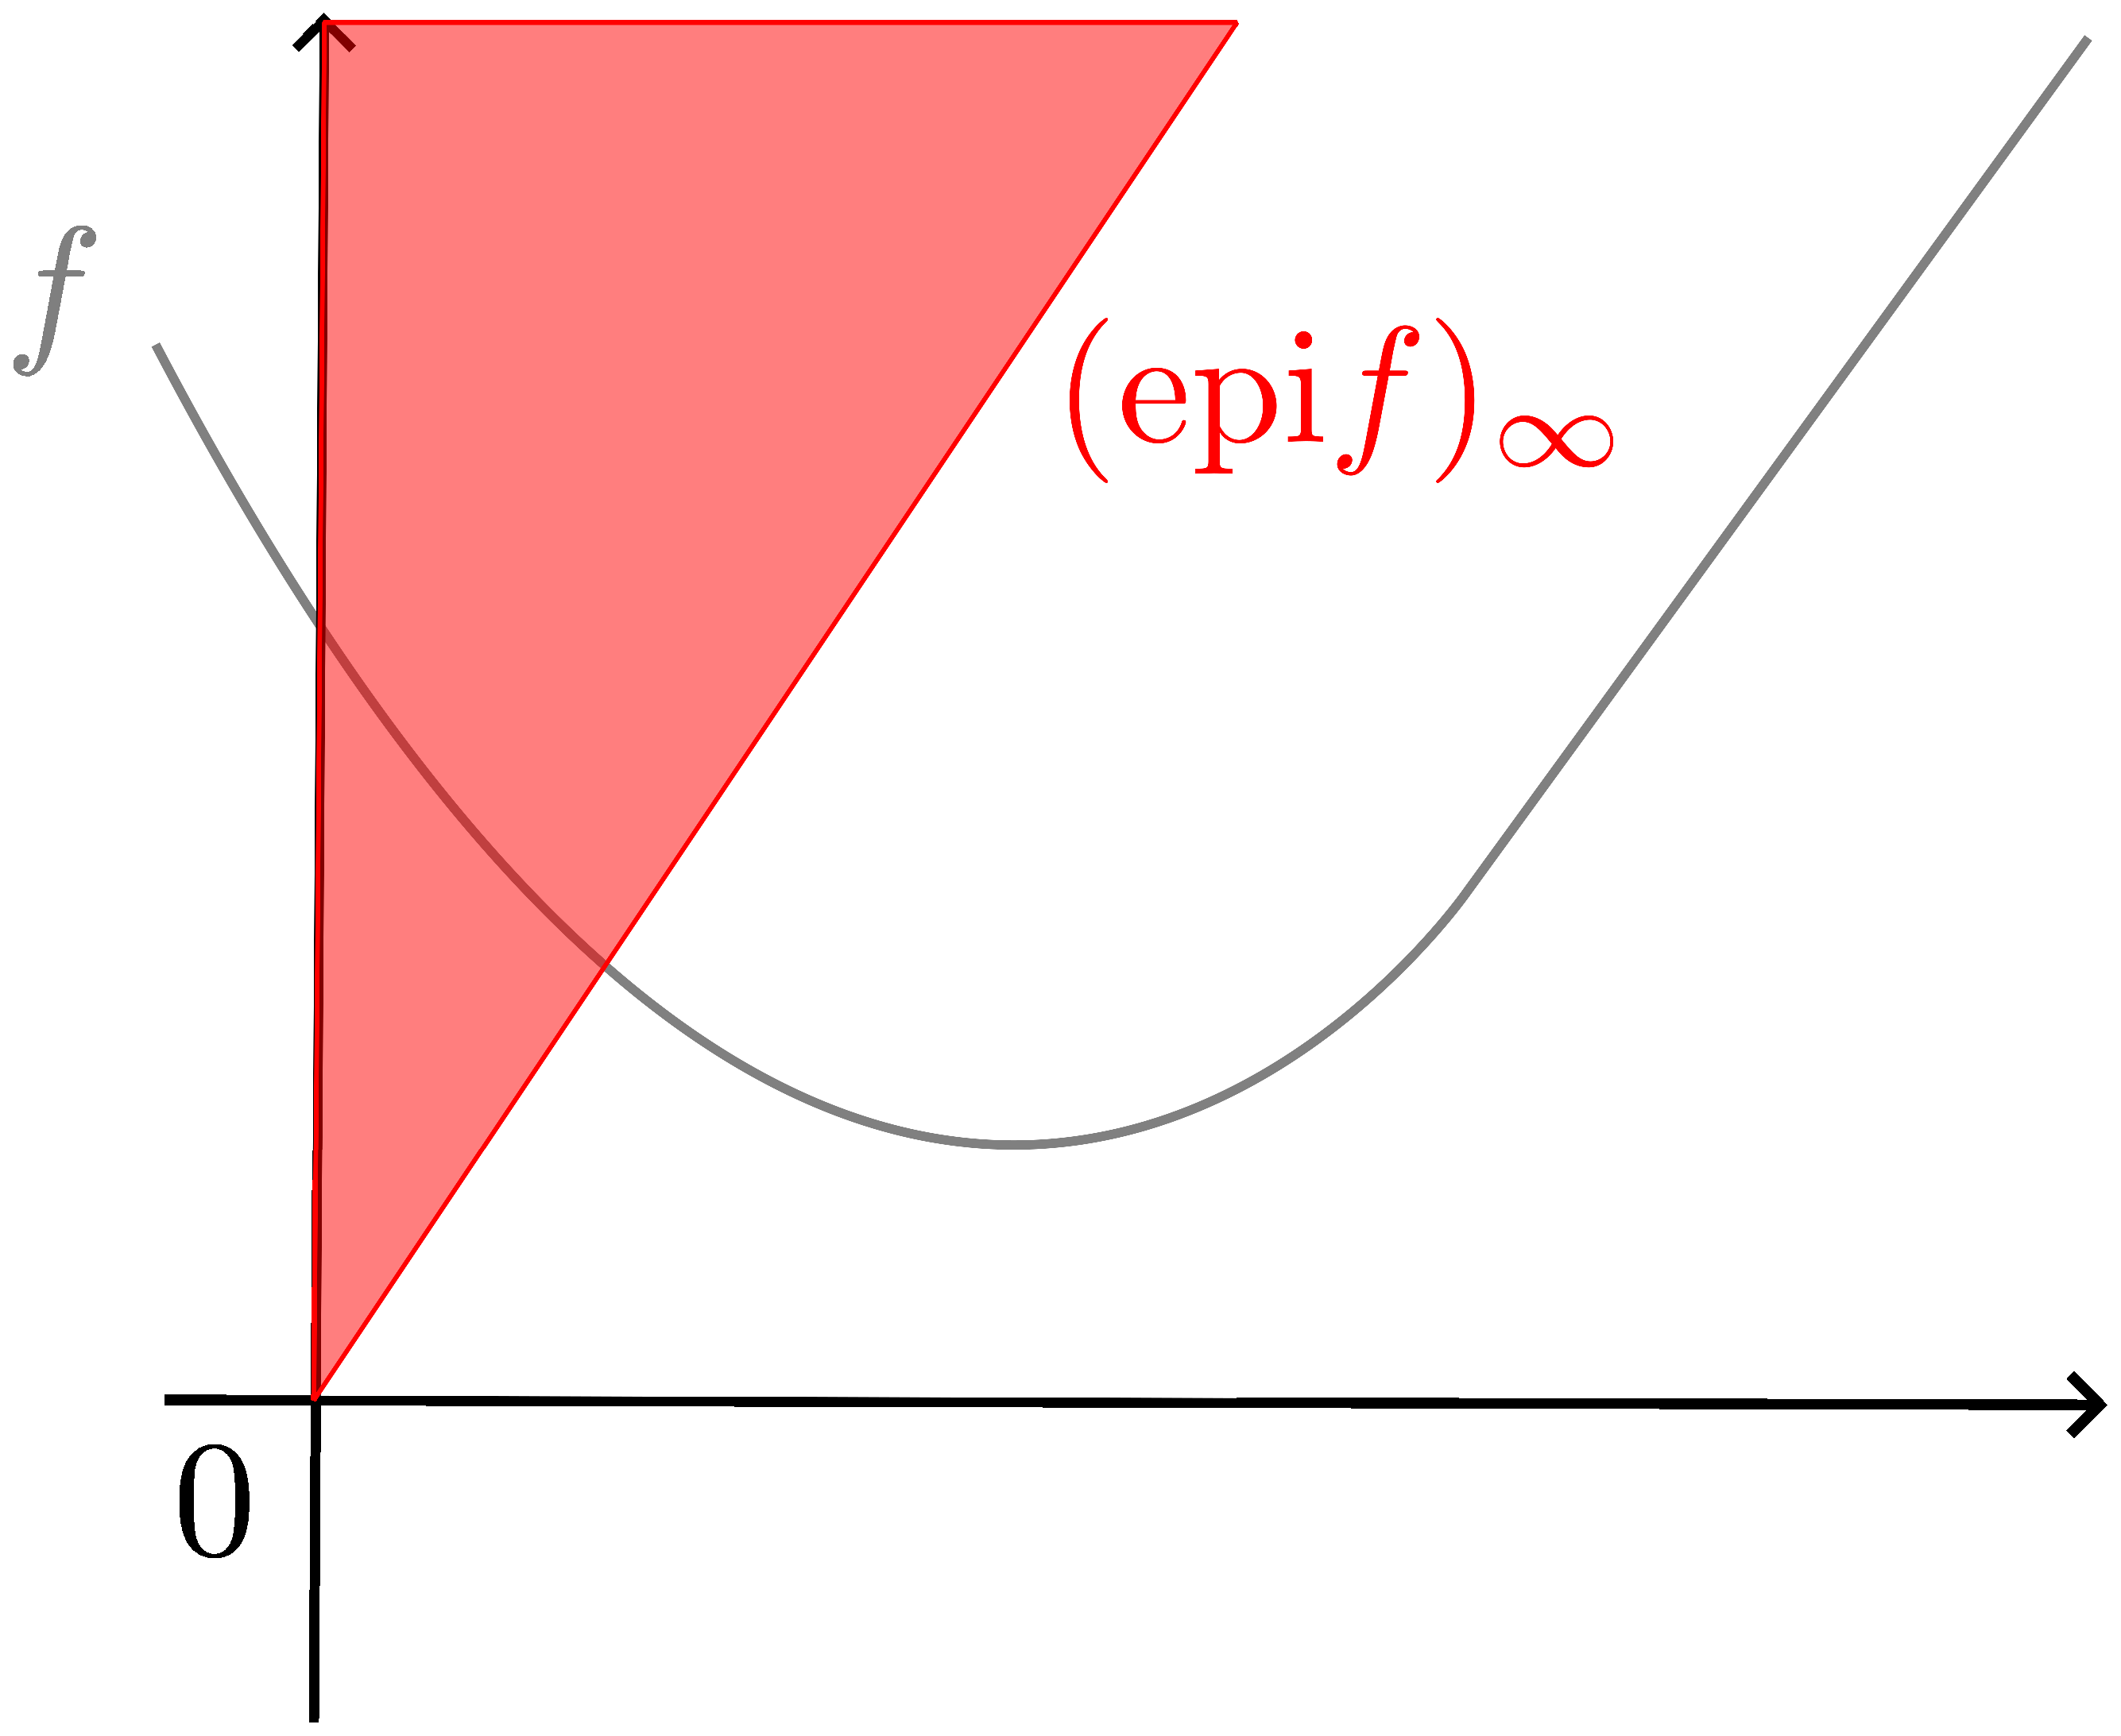
\includegraphics[keepaspectratio, scale=0.07]{figures/asymptotic_function_def/asymptotic_cone_epigraph_f.eps}
        \caption{(3) $(\Epigraph{f})_{\infty}$ の取得}
        \label{fill}
      \end{minipage} &
      \begin{minipage}[t]{0.45\hsize}
        \centering
        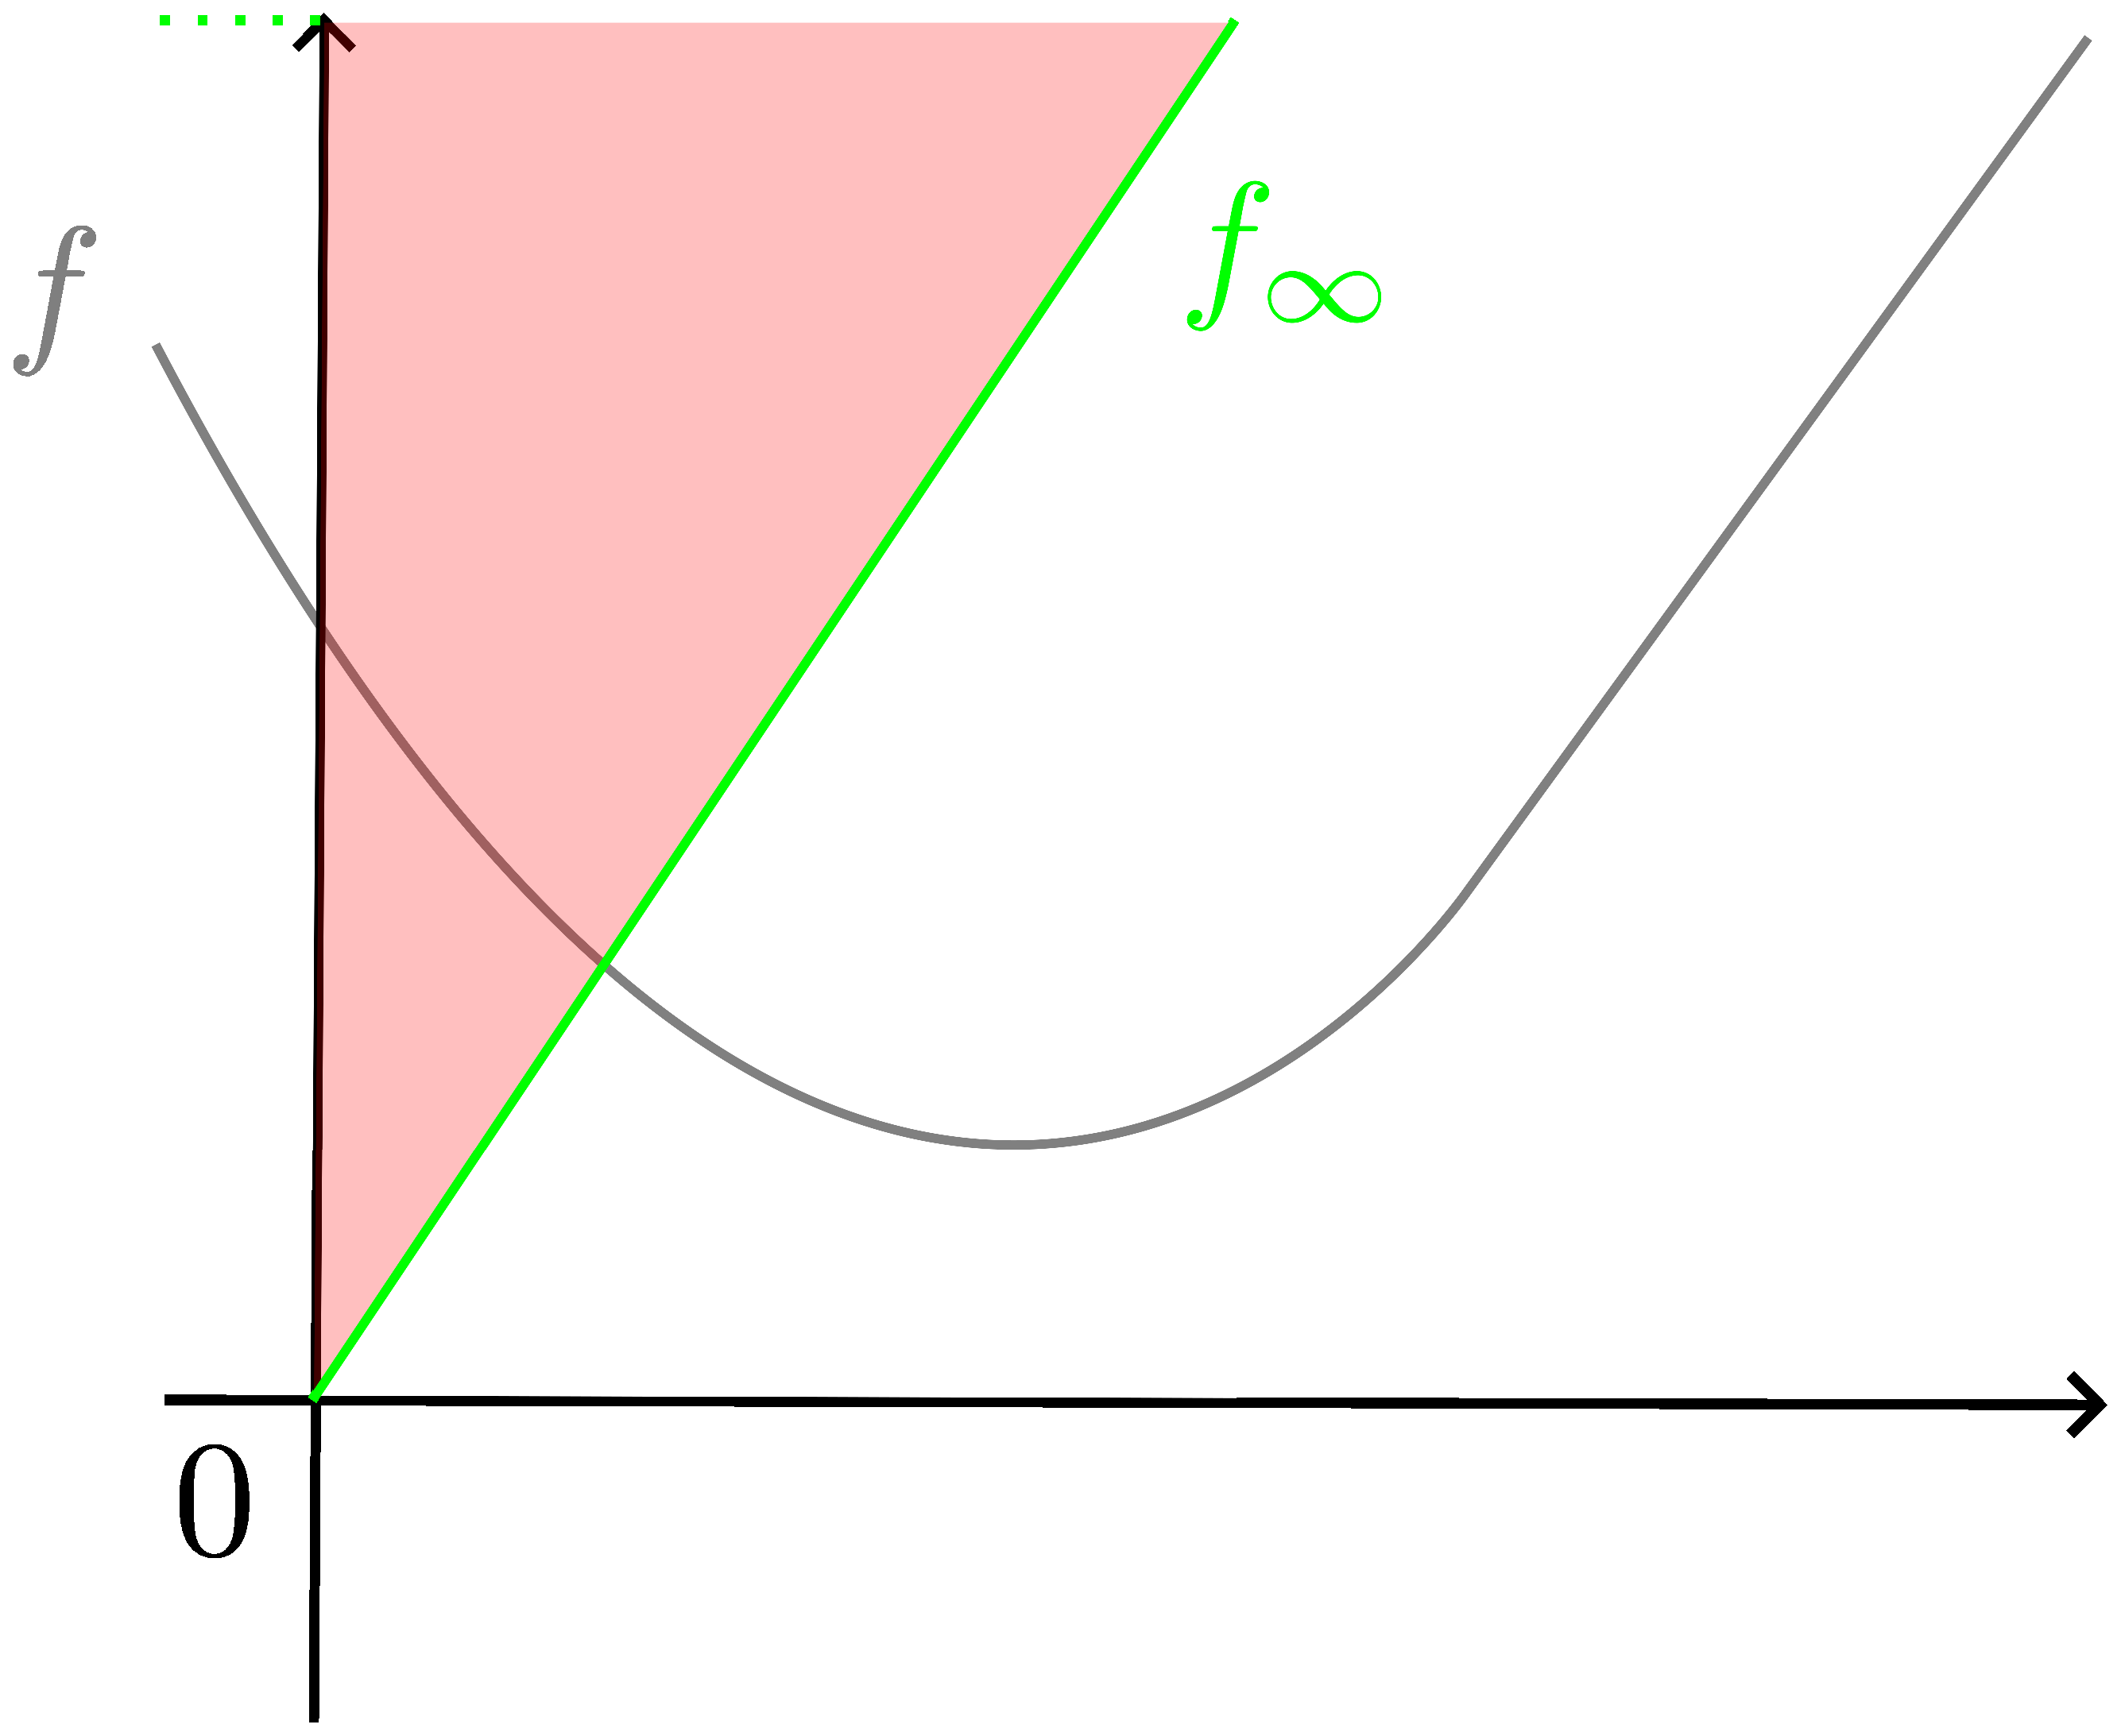
\includegraphics[keepaspectratio, scale=0.07]{figures/asymptotic_function_def/asymptotic_function_f.eps}
        \caption{(4) $f_{\infty}$ の定義}
        \label{transform}
      \end{minipage}
    \end{tabular}
  \end{figure}
\end{frame}

% 4.今後の研究
% ----------------------------------------------------------------
\section{今後の研究}
\begin{frame}{内容}
  \tableofcontents[currentsection]
\end{frame}

% 4.1
\begin{frame}{今後の研究}
  \begin{enumerate}
    \item 具体的な実数値関数の最適化問題に対して、Asymptotic Functions の考え方を適用する。
    \item Asymptotic Functions の考え方を集合値写像に拡張する。その際に、実数値関数で成り立っている性質が集合値写像においても成り立つかを確認する。
    \item 上の結果がどの程度の集合値写像の最適化問題に対して有効かを検証する。
  \end{enumerate}
\end{frame}

% 4.2
\begin{frame}{Asymptotic Functions の集合値写像への拡張(1)}
  実数値関数の場合、以下の4つの手順で Asymptotic Functions を定義した。これを集合値写像に対しても同様の手順で定義する。

  \begin{figure}[htbp]
    \begin{tabular}{cc}
      \begin{minipage}[t]{0.45\hsize}
        \centering
        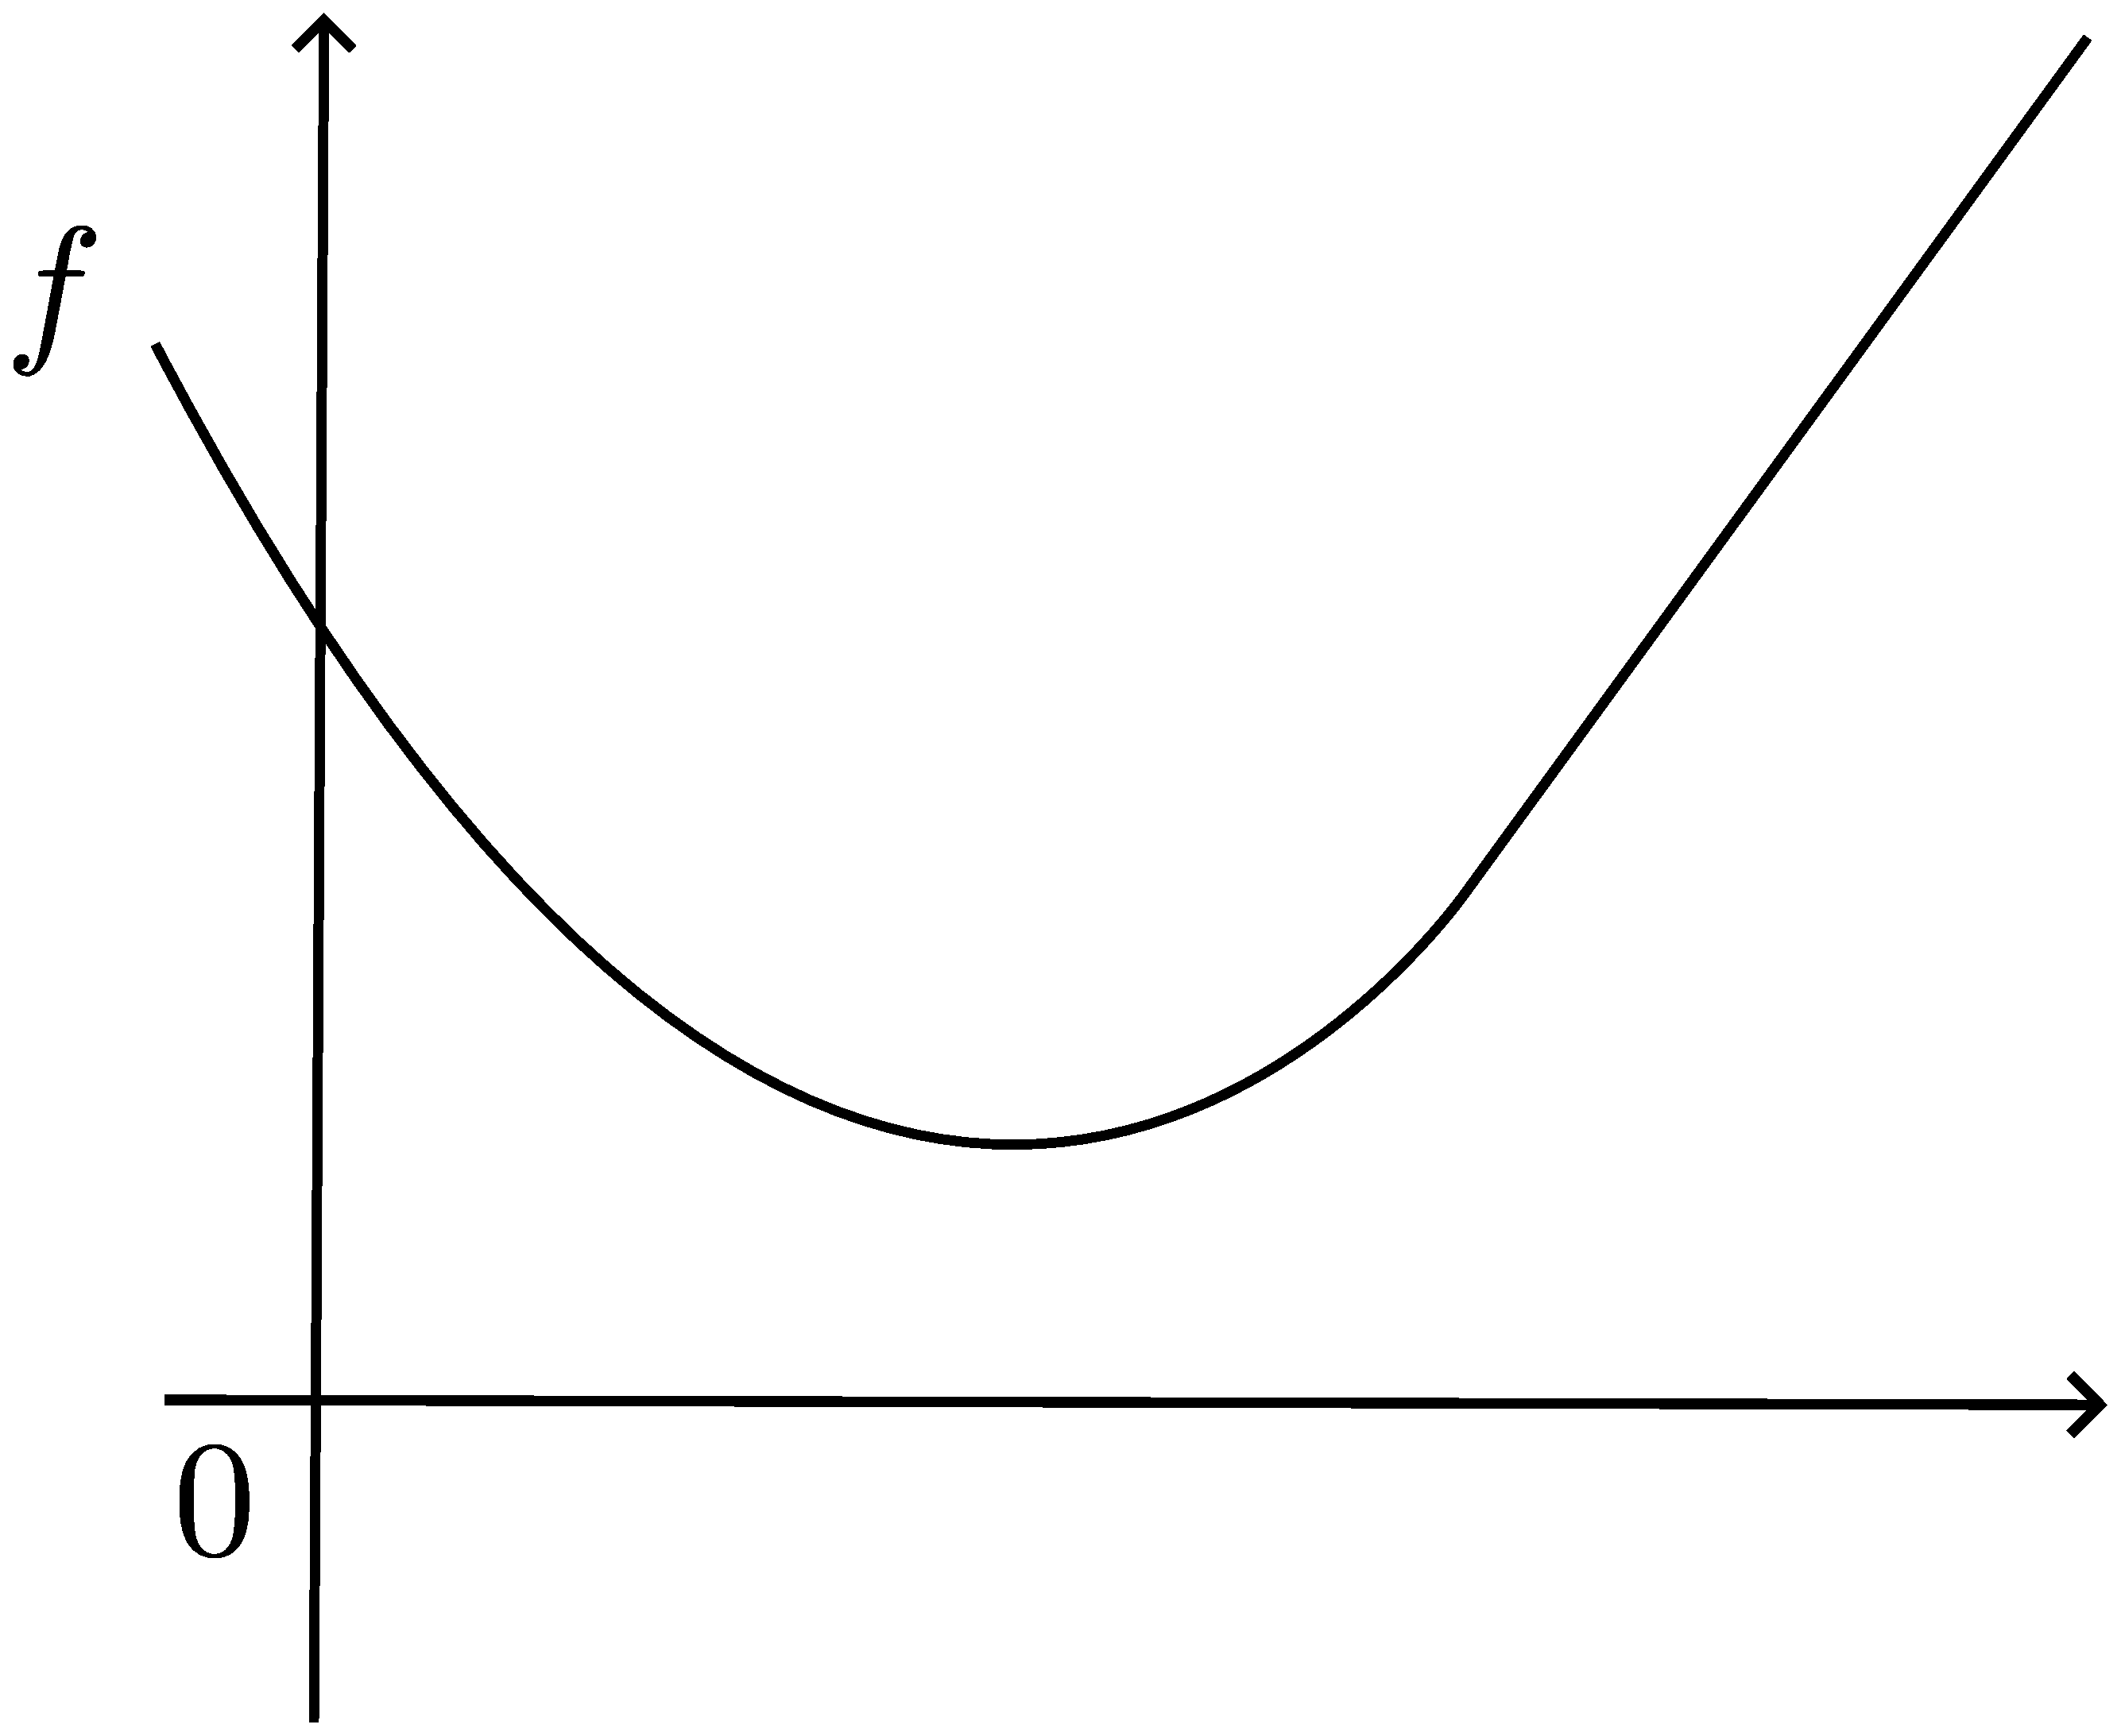
\includegraphics[keepaspectratio, scale=0.06]{figures/asymptotic_function_def/graph_base.eps}
        \caption{(1) $f$ の定義}
      \end{minipage} &
      \begin{minipage}[t]{0.45\hsize}
        \centering
        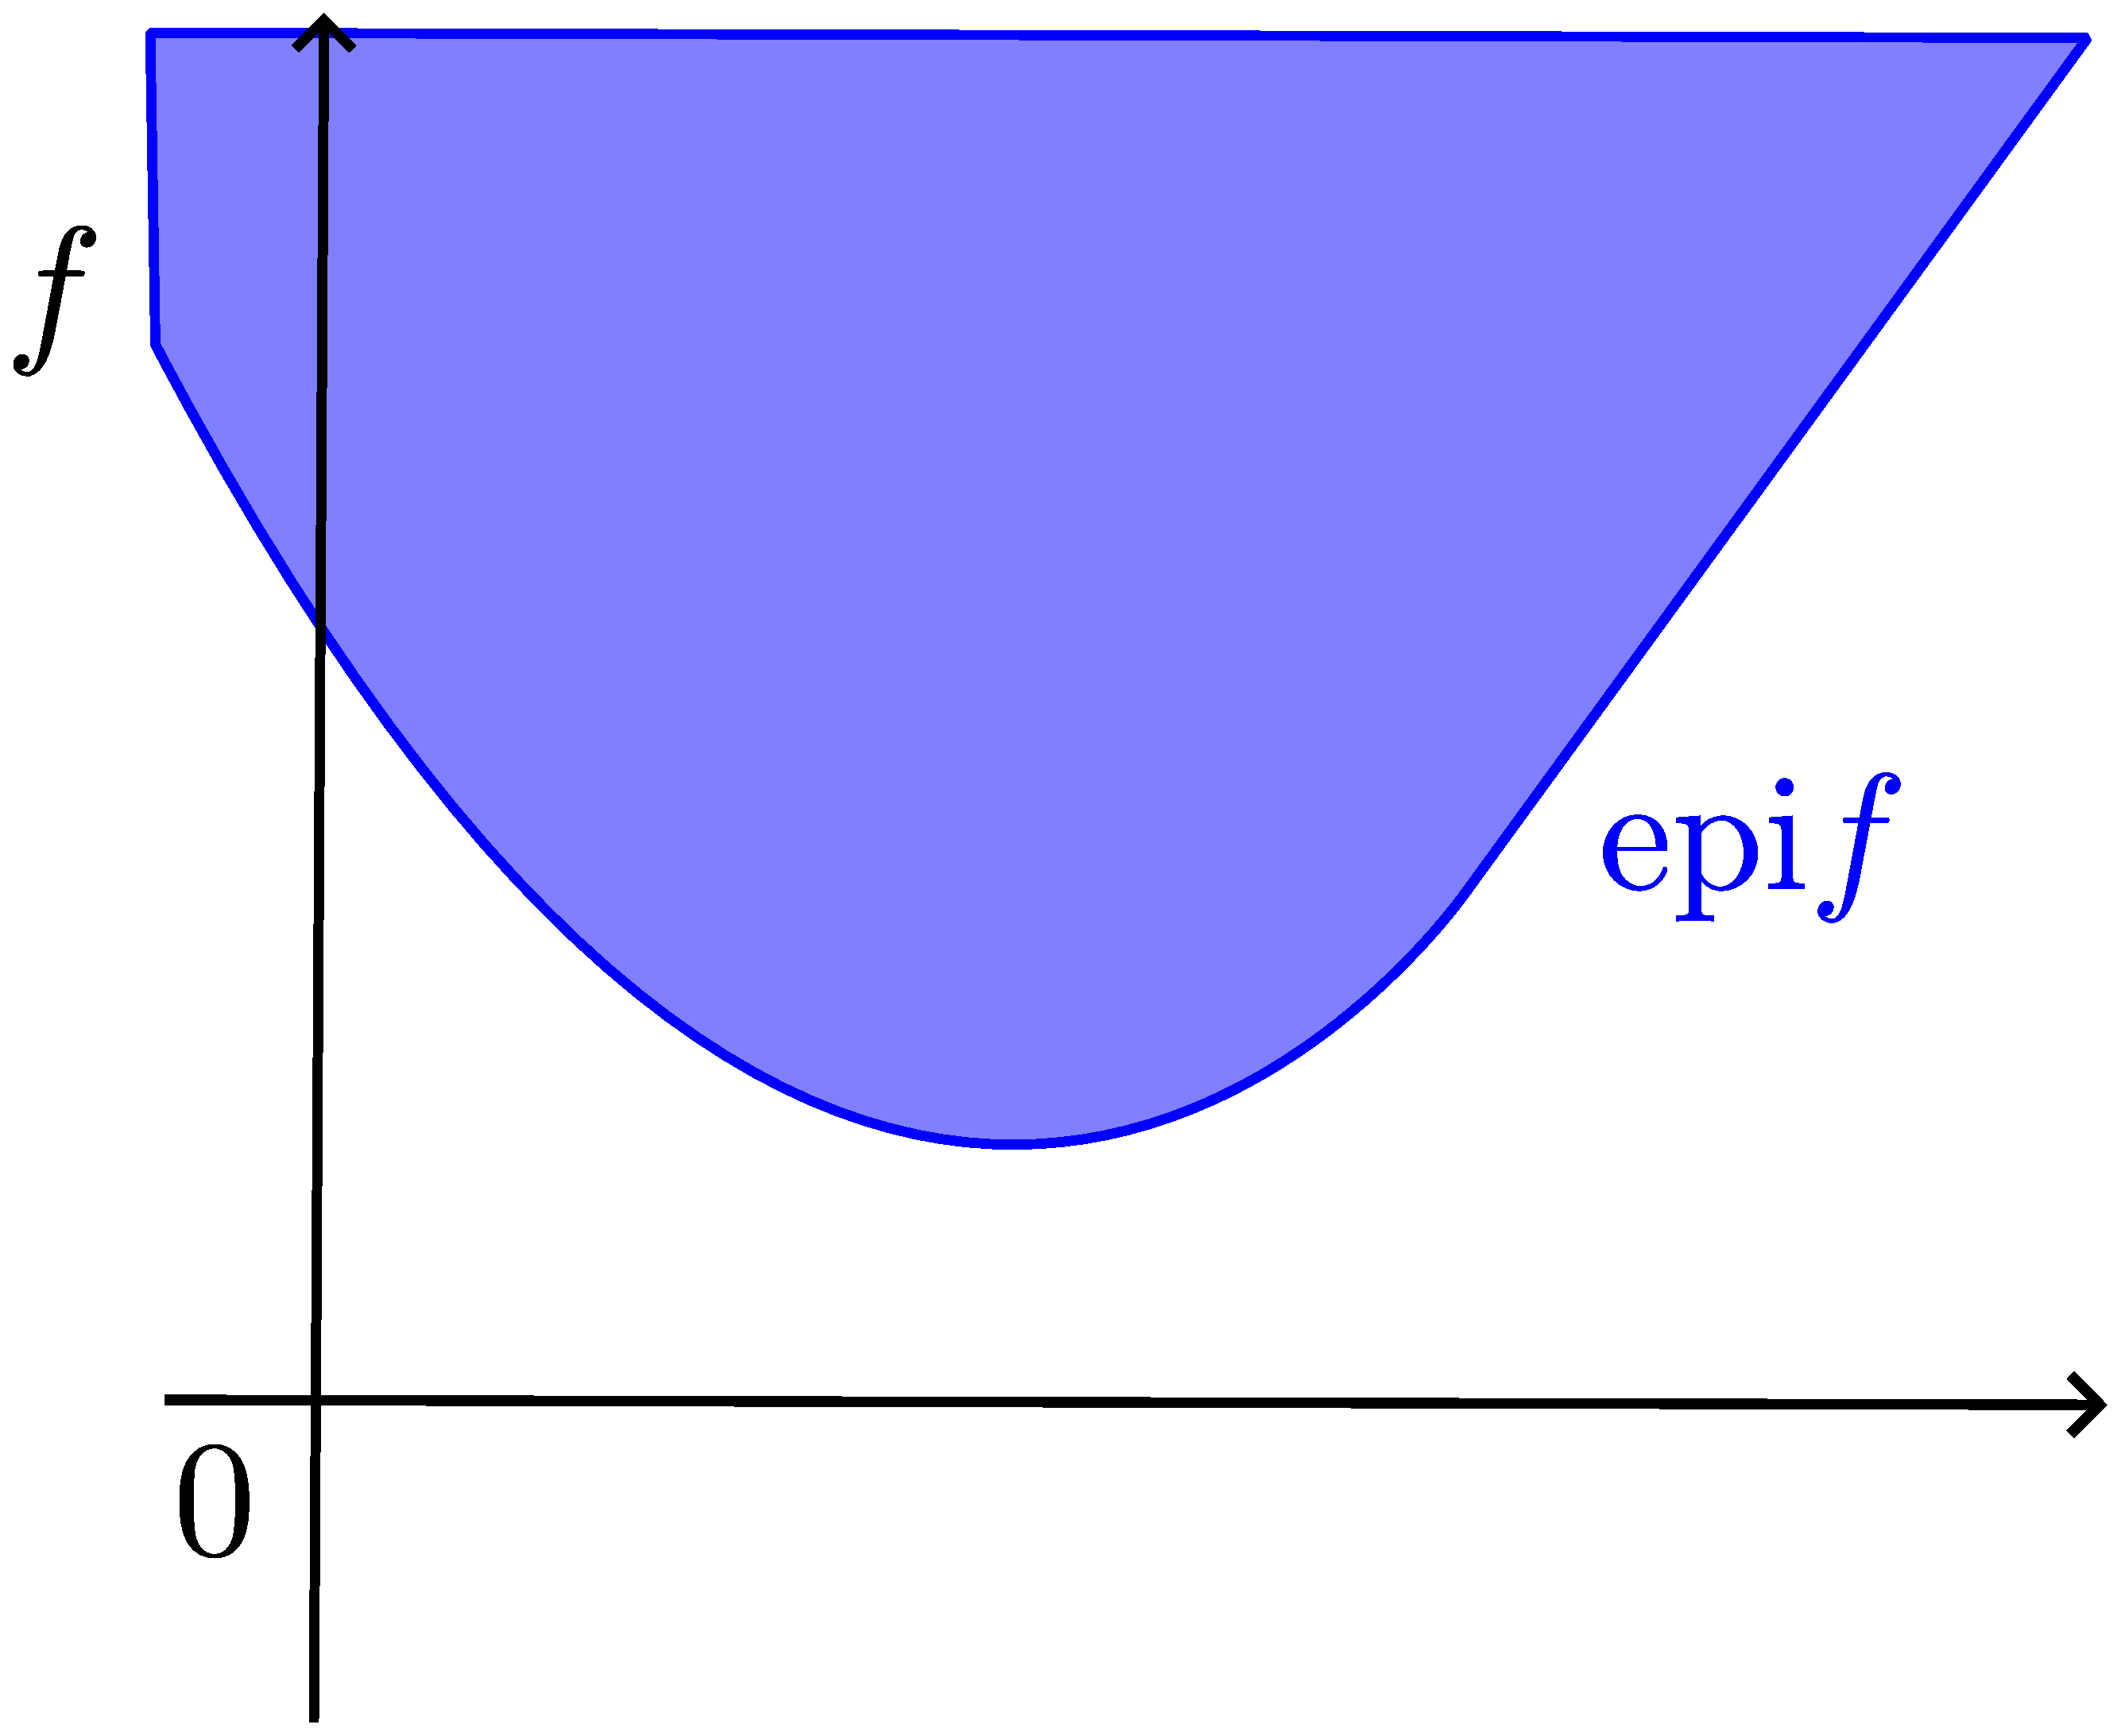
\includegraphics[keepaspectratio, scale=0.06]{figures/asymptotic_function_def/asymptotic_function_epigraph.eps}
        \caption{(2) $\Epigraph{f}$ の取得}
      \end{minipage} \\

      \begin{minipage}[t]{0.45\hsize}
        \centering
        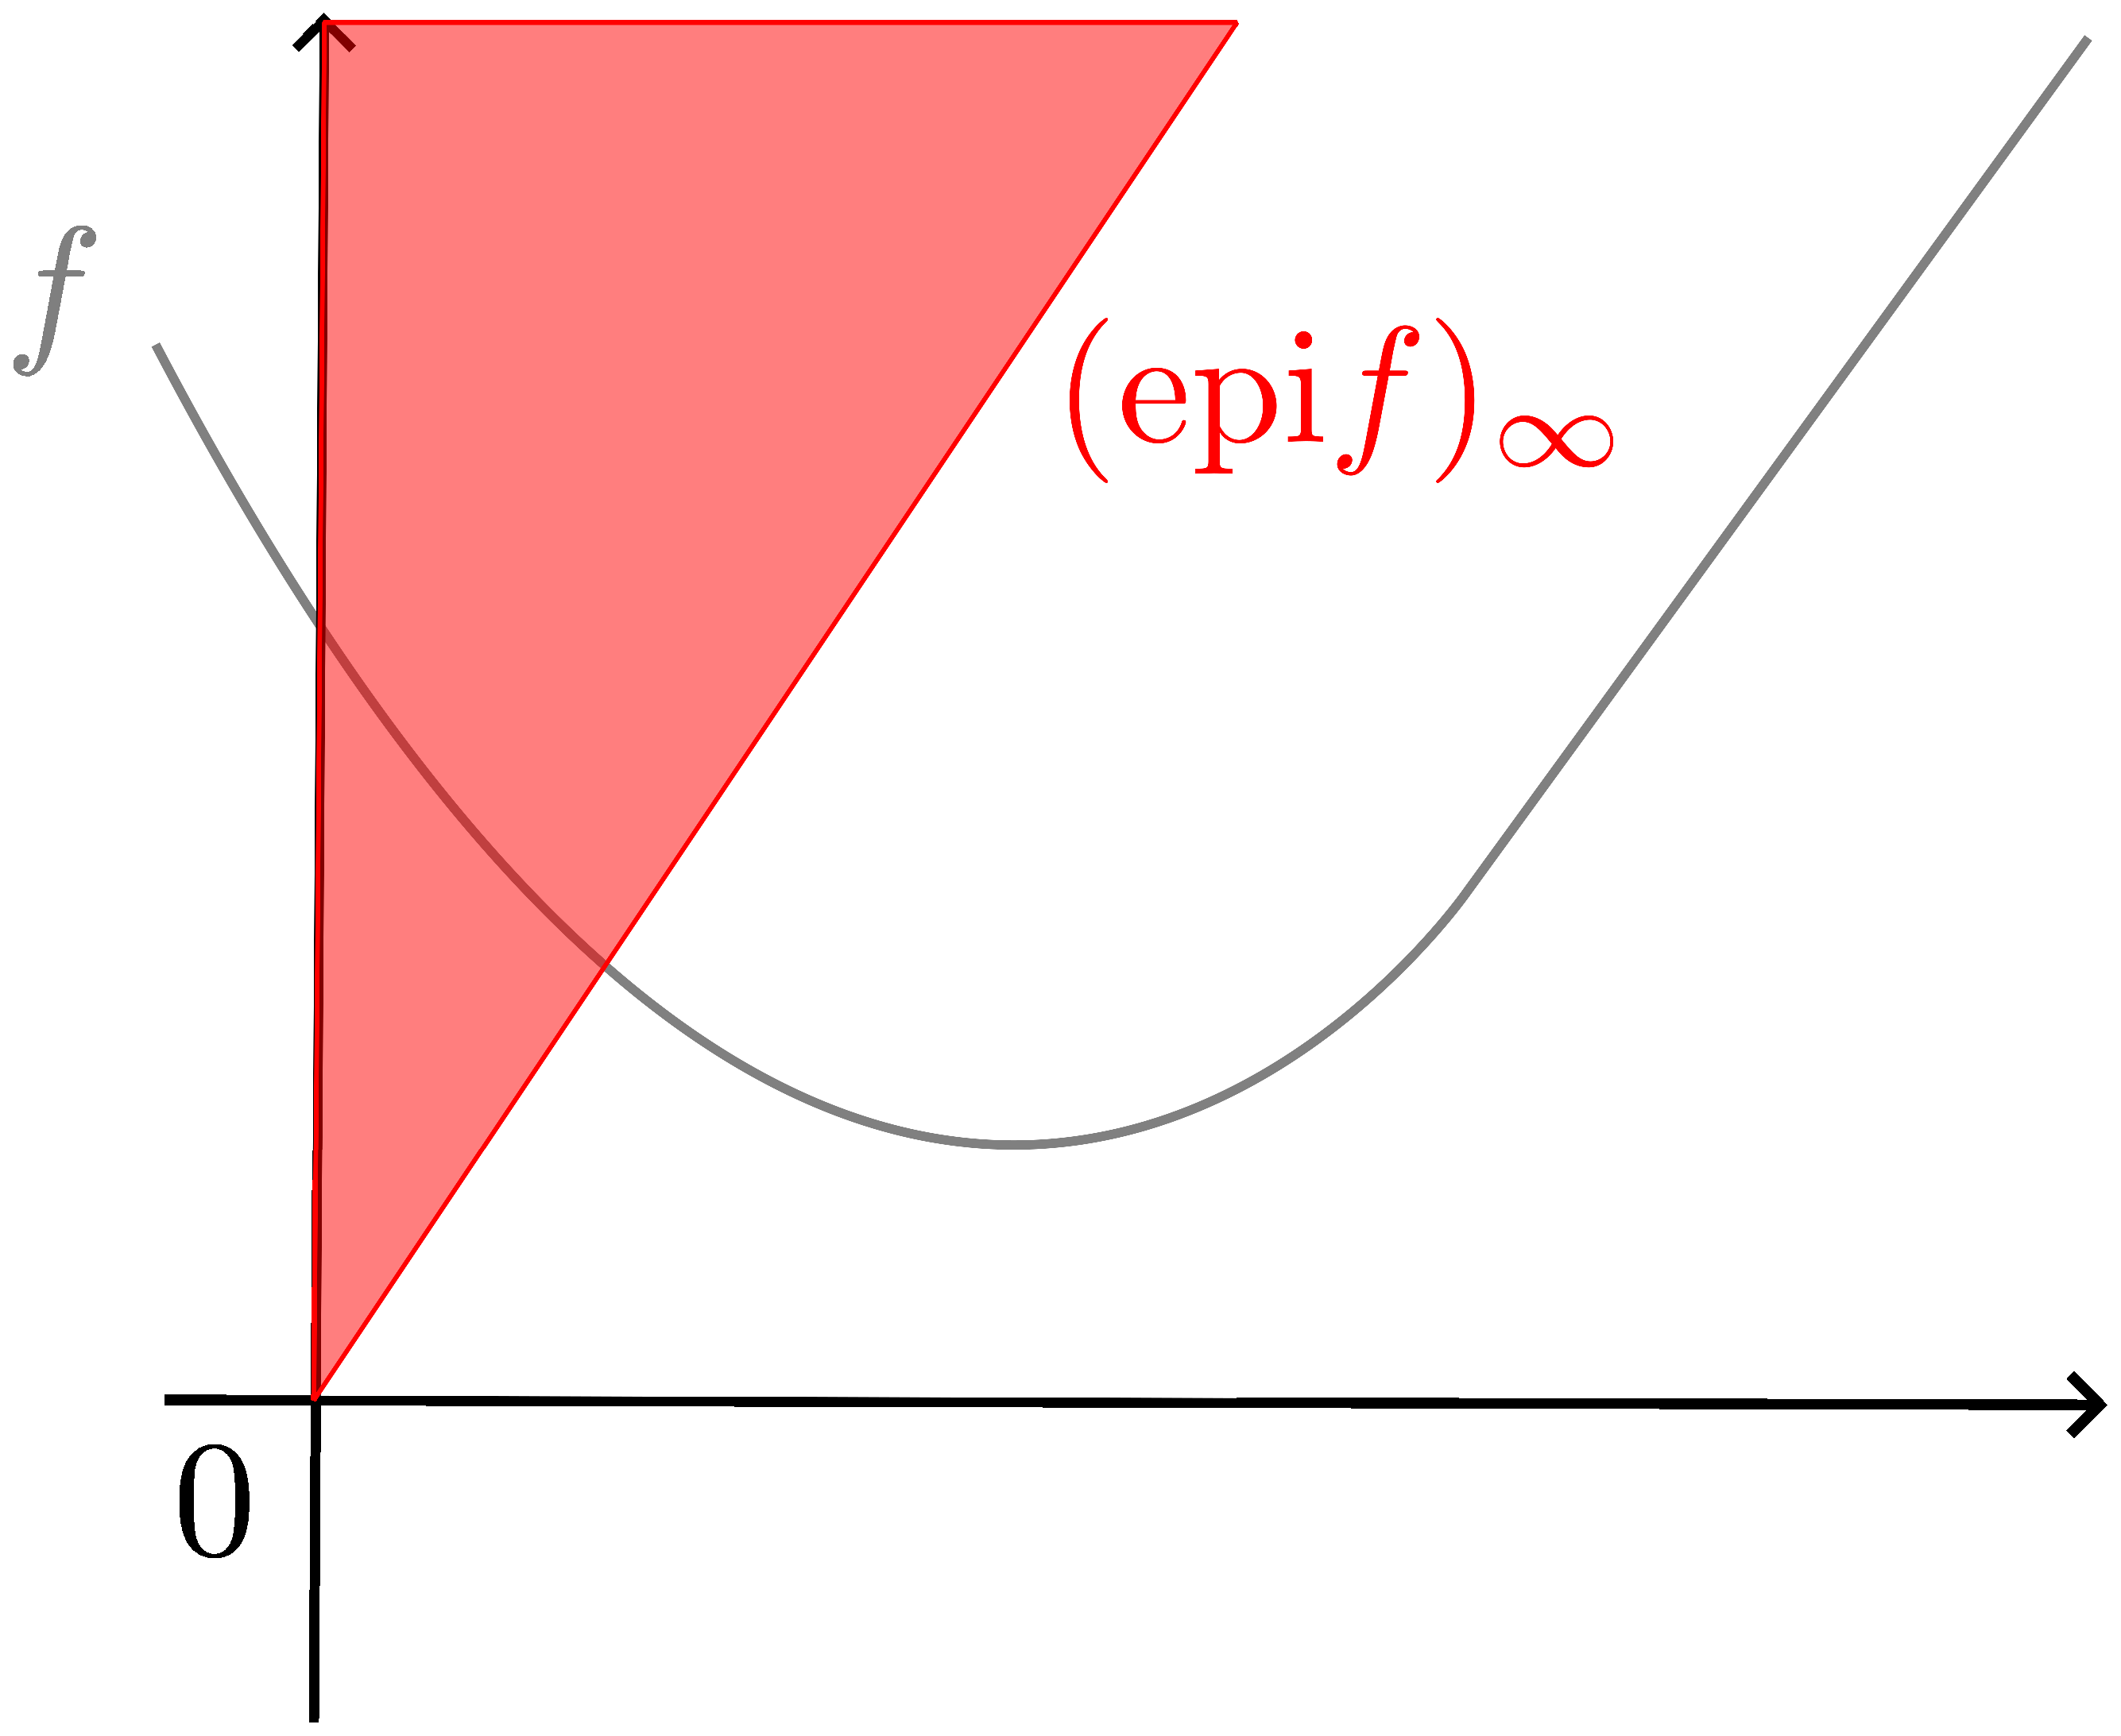
\includegraphics[keepaspectratio, scale=0.06]{figures/asymptotic_function_def/asymptotic_cone_epigraph_f.eps}
        \caption{(3) $(\Epigraph{f})_{\infty}$ の取得}
      \end{minipage} &
      \begin{minipage}[t]{0.45\hsize}
        \centering
        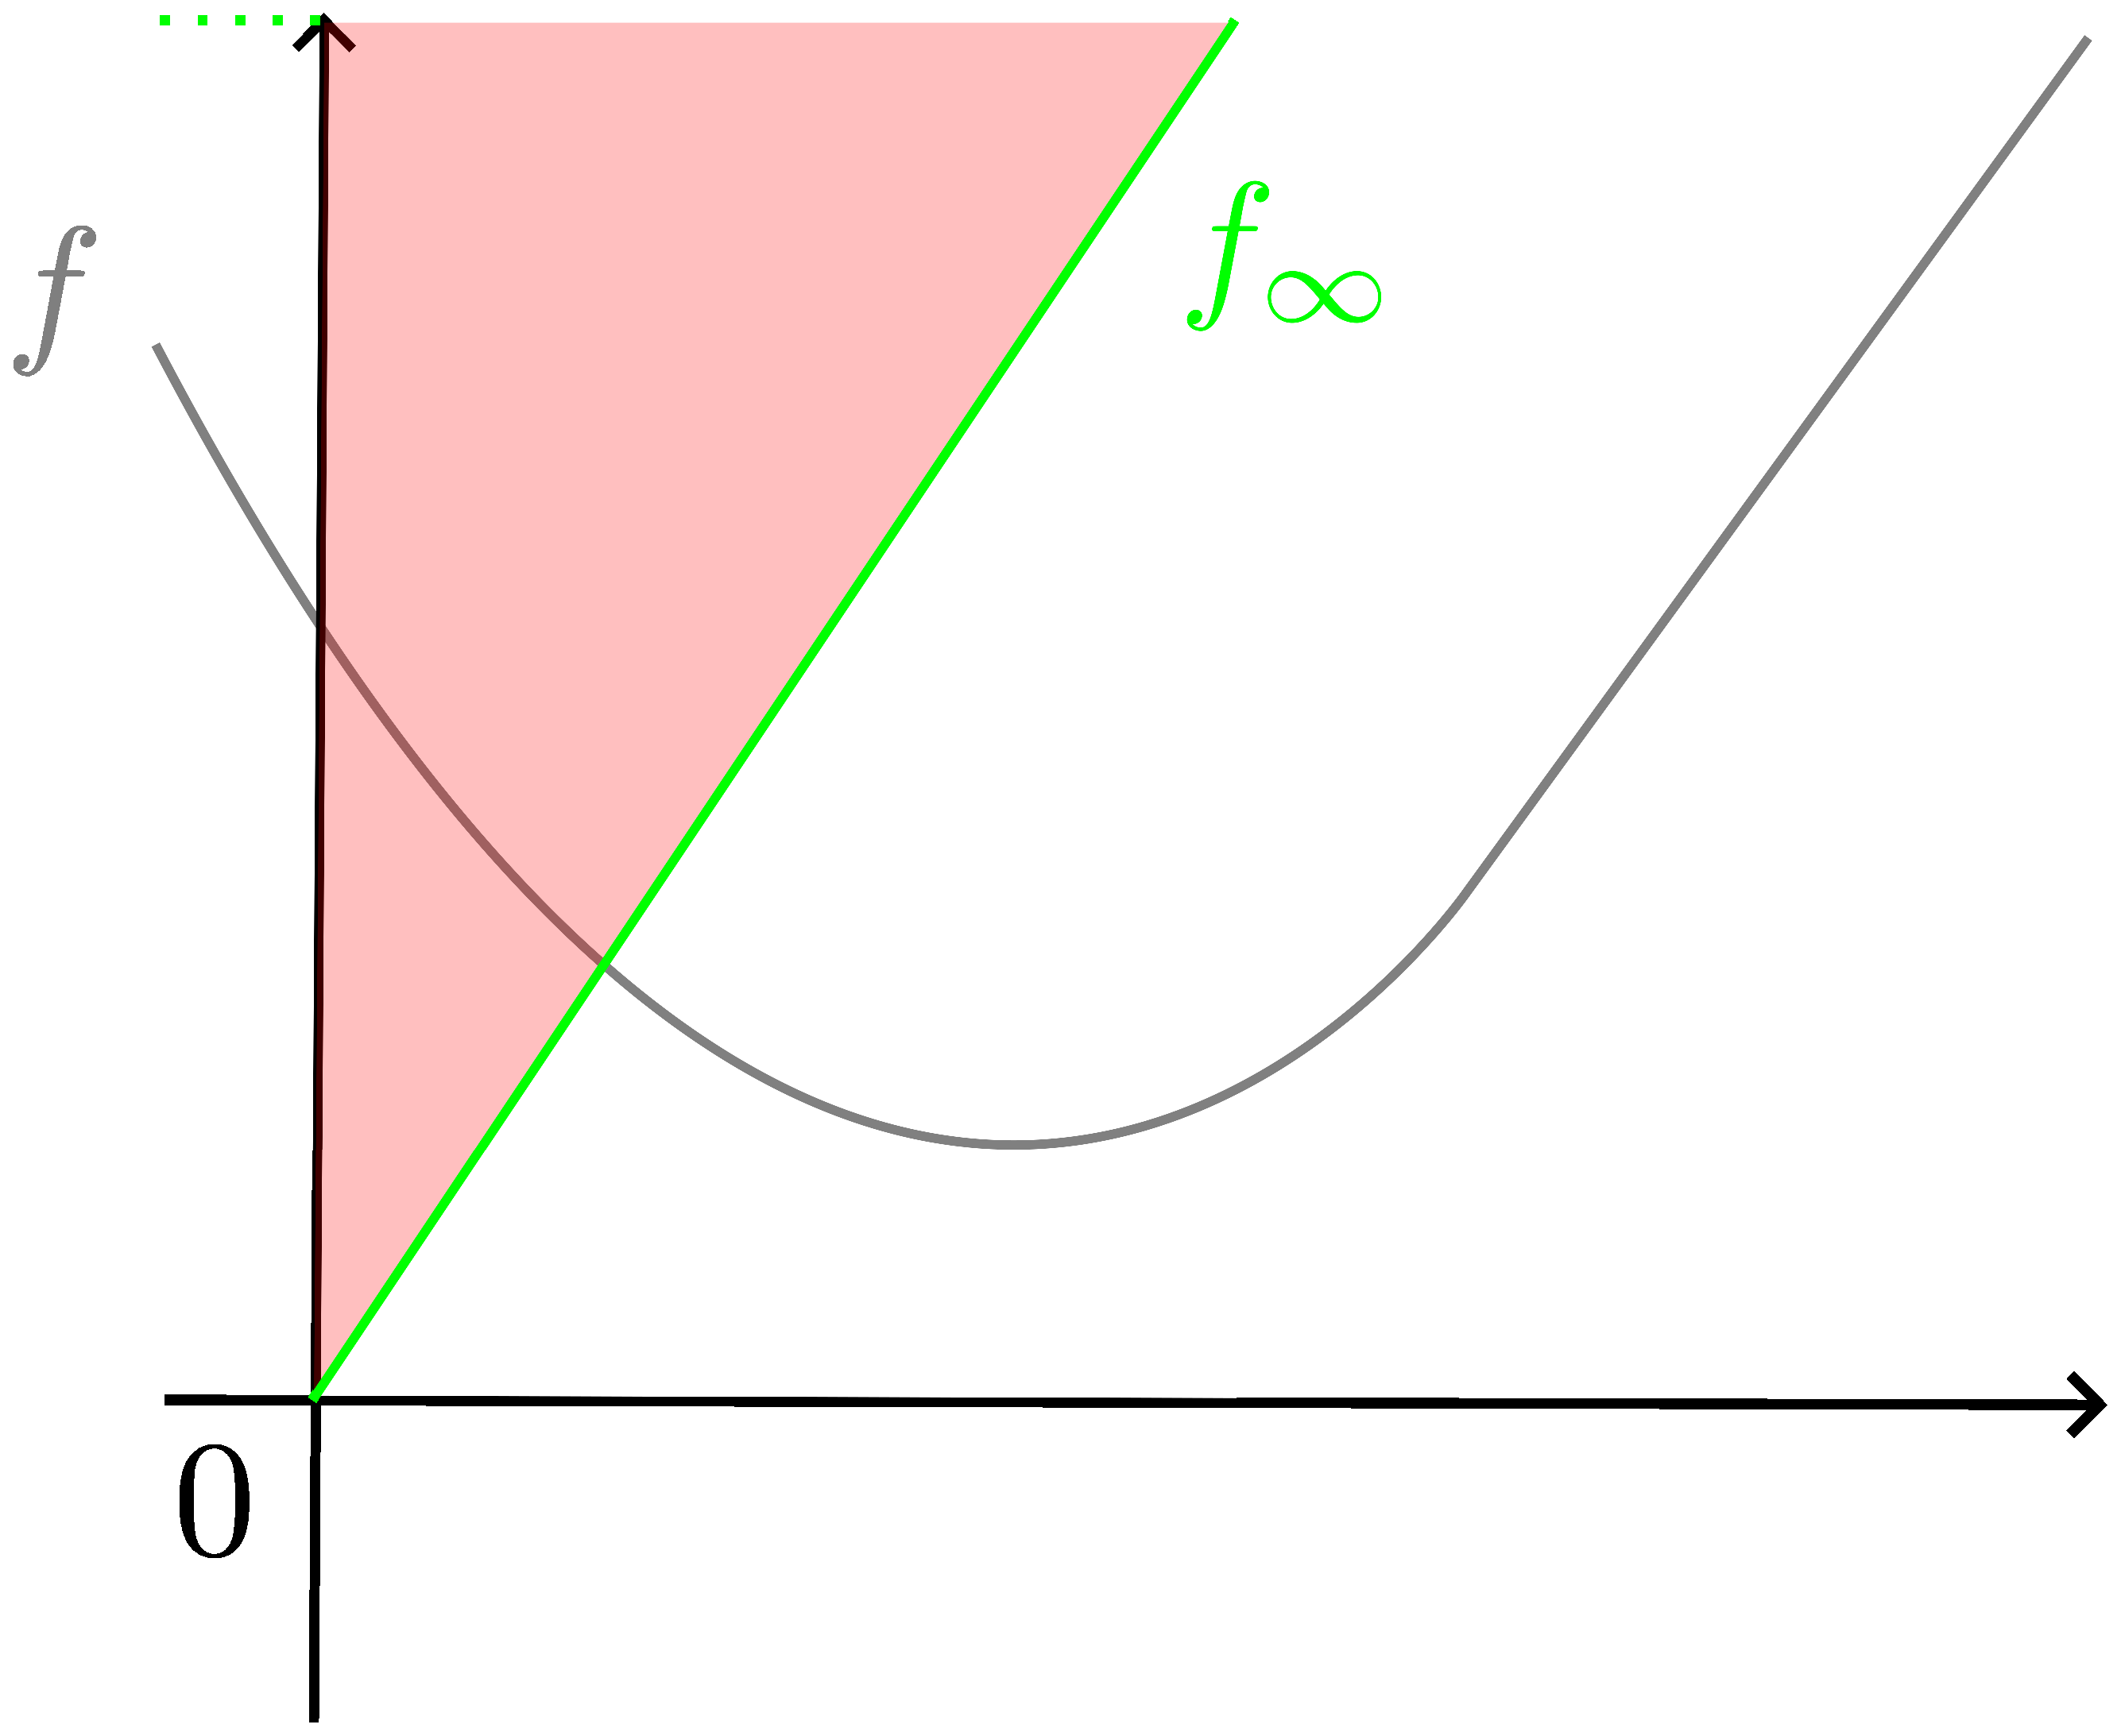
\includegraphics[keepaspectratio, scale=0.06]{figures/asymptotic_function_def/asymptotic_function_f.eps}
        \caption{(4) $f_{\infty}$ の定義}
      \end{minipage}
    \end{tabular}
  \end{figure}
\end{frame}

\begin{frame}{Asymptotic Functions の集合値写像への拡張(2)}
  集合値写像を以下のように定義します。

  \begin{block}{定義 5 (集合値写像) \cite{ref1}}
    $X, Y$ を非空集合とする。$X$ の各要素 $x$ に対して、$F(x) \in \mathcal{P}(Y)$ (この $\mathcal{P}(Y)$ は $Y$ の部分集合の族を表す) が定義されているとき、この $F$ を $X$ から $Y$ への集合値写像(Multifunction or Set-valued Maps)と呼ぶ。記号は、$F: X \rightarrow 2^Y$ で表す。
  \end{block}

  また、集合値写像に対する Proper の性質は以下のように定義します。

  \begin{block}{定義 6 (集合値写像に対する Proper) \cite{ref2}}
    $X, Y \ne \emptyset$, $F: X \rightarrow 2^Y$ とする。このとき、$\exists x_0 \in X \SuchThat F(x_0) \ne \emptyset$ が成り立つとき、$F$ は proper であるという。
  \end{block}
\end{frame}

\begin{frame}{Asymptotic Functions の集合値写像への拡張(3)}
  次に集合値写像に対しての Epigraph を以下のように定義します。

  \begin{block}{定義 7 (集合値写像に対する Epigraph) \cite{ref1}}
    $X, Y \ne \emptyset$, $F: X \rightarrow 2^Y$ とする。以下の集合を $F$ の Epigraph と呼ぶ。

    \begin{equation}
      \Epigraph{(F, \preccurlyeq )} \coloneqq \SetForm{(x,T) \in X \times \mathcal{P}(Y)}{F(x) \preccurlyeq T}. \notag
    \end{equation}
  \end{block}

  \begin{alertblock}{注意 2 (順序構造の選択)}
    上で登場した順序構造``$\preccurlyeq$''は、$\mathcal{P}(Y)$ 上の集合同士を比較する順序構造とする。
    現在は仮で``$\preccurlyeq$''としているが、後でこの順序構造をどのように選択するかを検討する必要がある。
  \end{alertblock}
\end{frame}

\begin{frame}{Asymptotic Functions の集合値写像への拡張(4)}
  集合に対する Asymptotic Cones を以下のように定義します。

  \begin{block}{定義 8 (集合族に対する Asymptotic Cones)}
    $Y \ne \emptyset$, $\mathcal{P}(Y)$ を $Y$ の部分集合の族とする。このとき$\mathcal{P}(Y)$ の asymptotic cone、記号では $(\mathcal{P}(Y))_\infty$ 、は集合列 $\{ Y_k \} \subset \mathcal{P}(Y)$ を用いて以下のように定義する。
    \begin{equation}
      (\mathcal{P}(Y))_\infty = \left\{ D \:\middle|\: \exists t_k \rightarrow +\infty, \exists Y_k \in \mathcal{P}(Y) \:\text{with}\: \limsup_{k \to \infty} \frac{Y_k}{t_k} = \liminf_{k \to \infty} \frac{Y_k}{t_k} = D \right\}. \notag
    \end{equation}
  \end{block}

  \begin{alertblock}{注意 3 (Asymptotic Functions の作成)}
    残りの課題として、集合族に対する Asymptotic Cones を考えた後、集合の inf のようなものを考える必要があり、この部分に関しても現在研究中。集合に強い順序関係を入れる or 何かしらのスカラー化関数を定義し、その尺度で集合の inf を考える、といった方法を考えている。
  \end{alertblock}
\end{frame}

% 4.References
% ----------------------------------------------------------------
\begin{frame}[t]{参考文献}
  \begin{itemize}
    \bibitem[1]{ref1}
    A. Alfred and M. Teboulle, asymptotic cones and functions in optimization and variational inequalities, Springer monographs in Mathematics, Springer-Verlag, New York, 2003.
    A. G\"{o}pfert, H. Riahi, C. Tammer, and C. Z\u{a}linescu, Variational methods in partially ordered spaces, vol.17 of CMS Books in Mathematics, Springer-Verlag, New York, 2003.
    \bibitem[2]{ref2}
    A. G\"{o}pfert, H. Riahi, C. Tammer, and C. Z\u{a}linescu, Variational methods in partially ordered spaces, vol.17 of CMS Books in Mathematics, Springer-Verlag, New York, 2003.
  \end{itemize}
\end{frame}

\end{document}
